% PLANTILLA PARA TRABAJOS EN LATEX
% Autor: Manuel Gachs Ballegeer
% GitHub: https://github.com/Manuelbelgicano
% Licencia: GNU General Public License v3.0
% Versión: 0.2

\documentclass[12pt,twoside,titlepage,a4paper]{article}

%%%%%%%%%%%%%%%%%%%%%%%%%%%%%%%%%%%%%%%%%
%			   COLORINES				%
%%%%%%%%%%%%%%%%%%%%%%%%%%%%%%%%%%%%%%%%%
\usepackage{xcolor}
% COLORES DE LA ESTRUCTURA DEL DOCUMENTO
\definecolor{ed_1}{HTML}{8A0808} % Portada
\definecolor{ed_2}{HTML}{FFFFFF} % Texto de la portada
\definecolor{ed_3}{HTML}{8A0808} % Títulos de las secciones
\definecolor{ed_4}{HTML}{610505} % Títulos de las subsecciones
\definecolor{ed_5}{HTML}{300303} % Títulos de las subsubsecciones
\definecolor{ed_6}{HTML}{610B0B} % Texto del encabezado
% COLORES PARA MATEMÁTICAS
\definecolor{m_1}{HTML}{8A0808} % Teoremas, lemas
\definecolor{m_2}{HTML}{610505} % Definiciones
\definecolor{m_3}{HTML}{300303} % Corolarios
\definecolor{m_4}{HTML}{000000} % Ejemplos, demostraciones
% COLORES PARA CÓDIGO
\definecolor{c_1}{HTML}{8A0808} % Línea a la izquierda
\definecolor{c_2}{HTML}{610B0B} % Palabras reservadas
\definecolor{c_3}{HTML}{B40431} % Cadenas de caracteres
\definecolor{c_4}{HTML}{333333} % Comentarios
% COLORES PARA LISTAS
\definecolor{l_1}{HTML}{8A0808} % Primer símbolo
\definecolor{l_2}{HTML}{610505} % Primera indentación
\definecolor{l_3}{HTML}{300303} % Segunda indentación
\definecolor{l_4}{HTML}{000000} % Tercera indentación
% COLORES PARA MARCOS
\definecolor{ma_1}{HTML}{8A0808} % Línea marco ejemplos
\definecolor{ma_2}{HTML}{610505} % Línea marco notas
\definecolor{ma_3}{HTML}{FFEDEE} % Fondo ejemplos
\definecolor{ma_4}{HTML}{FFE0DF} % Fondo notas

%%%%%%%%%%%%%%%%%%%%%%%%%%%%%%%%%%%%%%%%%
%				  MARCOS				%
%%%%%%%%%%%%%%%%%%%%%%%%%%%%%%%%%%%%%%%%%
\usepackage[xcolor]{mdframed} % Marcos
\mdfsetup{ % Configuración general de los marcos
  skipabove=1em, % Espacio sobre los marcos
  skipbelow=1em, % Espacio bajo los marcos
  innertopmargin=0.3em, % Margen interior superior
  innerbottommargin=1em, % Margen interior inferior
  splittopskip=2\topsep, % Espacio entre marcos
  usetwoside=false, % Diferenciar páginas
}

\mdfdefinestyle{marco_ejemplos}{ % Nombre del estilo
	linewidth=2pt, % Grosor de la línea
	linecolor=ma_1, % Color de la línea
	backgroundcolor=ma_3, % Color de fondo
	topline=false, % Línea arriba
	leftline=true, % Línea a la izquierda
	bottomline=false, % Línea abajo
	rightline=false,% Línea a la derecha
	leftmargin=0em, % Margen a la izquierda
	innerleftmargin=1em, % Margen interior a la izquierda
	innerrightmargin=1em, % Margen interior a la derecha
	rightmargin=0em, % Margen a la derecha
}
\mdfdefinestyle{marco_anotaciones}{ % Nombre del estilo
	linewidth=1pt, % Grosor de la línea
	linecolor=ma_2, % Color de la línea
	backgroundcolor=ma_4, % Color de fondo
	topline=true, % Línea arriba
	leftline=true, % Línea a la izquierda
	bottomline=true, % Línea abajo
	rightline=true,% Línea a la derecha
	leftmargin=0em, % Margen a la izquierda
	innerleftmargin=1em, % Margen interior a la izquierda
	innerrightmargin=1em, % Margen interior a la derecha
	rightmargin=0em, % Margen a la derecha
}

%%%%%%%%%%%%%%%%%%%%%%%%%%%%%%%%%%%%%%%%%
%			  MATEMÁTICAS				%
%%%%%%%%%%%%%%%%%%%%%%%%%%%%%%%%%%%%%%%%%
\usepackage{amsmath} % Matemáticas
\usepackage{amsfonts} % Letras caligráficas para matemáticas
\usepackage{mathtools} % Matemáticas extra
\usepackage{amsthm} % Teoremas
\renewenvironment{proof}{{\bfseries\color{m_4}Demostración:}}{\qed} % Cambiar el título de las demostraciones
% ESTILOS DE TEOREMAS
\newtheoremstyle{teorema} % Nombre del estilo
{} % Espacio por encima
{} % Espacio por debajo
{} % Estilo del cuerpo
{} % Indentación
{\color{m_1}\bfseries} % Estilo de la cabecera
{:} % Símbolo tras la cabecera
{ } % Espacio tras la cabecera
{} % Especificación de la cabecera
\newtheoremstyle{lema} % Nombre del estilo
{} % Espacio por encima
{} % Espacio por debajo
{} % Estilo del cuerpo
{} % Indentación
{\color{m_1}\bfseries} % Estilo de la cabecera
{:} % Símbolo tras la cabecera
{ } % Espacio tras la cabecera
{} % Especificación de la cabecera
\newtheoremstyle{definicion} % Nombre del estilo
{} % Espacio por encima
{} % Espacio por debajo
{} % Estilo del cuerpo
{} % Indentación
{\color{m_2}\bfseries} % Estilo de la cabecera
{:} % Símbolo tras la cabecera
{ } % Espacio tras la cabecera
{} % Especificación de la cabecera
\newtheoremstyle{corolario} % Nombre del estilo
{} % Espacio por encima
{} % Espacio por debajo
{} % Estilo del cuerpo
{} % Indentación
{\color{m_3}\bfseries} % Estilo de la cabecera
{:} % Símbolo tras la cabecera
{ } % Espacio tras la cabecera
{} % Especificación de la cabecera
\newtheoremstyle{nota} % Nombre del estilo
{} % Espacio por encima
{} % Espacio por debajo
{\itshape} % Estilo del cuerpo
{} % Indentación
{\color{m_4}\bfseries} % Estilo de la cabecera
{:} % Símbolo tras la cabecera
{ } % Espacio tras la cabecera
{} % Especificación de la cabecera
\newtheoremstyle{ejemplo} % Nombre del estilo
{} % Espacio por encima
{} % Espacio por debajo
{} % Estilo del cuerpo
{} % Indentación
{\color{m_4}\itshape\bfseries} % Estilo de la cabecera
{ } % Símbolo tras la cabecera
{ } % Espacio tras la cabecera
{} % Especificación de la cabecera
% COMANDOS
% Eliminar '*' para añadir numeración a los lemas, teoremas...
\theoremstyle{definicion}
\newtheorem*{defi}{Definición} % Comando para las definiciones
\theoremstyle{lema}
\newtheorem*{lem}{Lema} % Comando para los lemas
\theoremstyle{teorema}
\newtheorem*{teo}{Teorema} % Comando para los teoremas
\theoremstyle{corolario}
\newtheorem*{cor}{Corolario} % Comando para los corolarios
\theoremstyle{ejemplo}
\newtheorem*{eje}{} % Comando para los ejemplos
\theoremstyle{nota}
\newtheorem*{ano}{Nota} % Comando para las anotaciones
\surroundwithmdframed[style=marco_ejemplos]{eje}
\surroundwithmdframed[style=marco_anotaciones]{ano}

%%%%%%%%%%%%%%%%%%%%%%%%%%%%%%%%%%%%%%%%%
%			   TIPOGRAFÍA				%
%%%%%%%%%%%%%%%%%%%%%%%%%%%%%%%%%%%%%%%%%
\usepackage[sfdefault]{cabin}
\usepackage[T1]{fontenc}

%%%%%%%%%%%%%%%%%%%%%%%%%%%%%%%%%%%%%%%%%
%				  CÓDIGO				%
%%%%%%%%%%%%%%%%%%%%%%%%%%%%%%%%%%%%%%%%%
\usepackage{listingsutf8}
\lstset{
	inputencoding=utf8/latin1, % Codificación
	xleftmargin=1em, % Margen extra a la izquierda
	breaklines=true, % Romper líneas largas
	language=XML, % Lenguaje del código
	frame=single, % Enmarcado
	numbers=none, % Números de línea
	numbersep=8pt, % Separación de los números de línea
	tabsize=4, % Tamaño de los tabs
	frame=leftline, % Posición del enmarcado
	framerule=2pt, % Grosor del enmarcado
	showstringspaces=false, % Mostrar los espacios en las cadenas de caracteres
	basicstyle=\footnotesize\ttfamily, % Estilo del código
	numberstyle=\normalfont, % Estilo de los números de línea
	rulecolor=\color{c_1}, % Estilo del enmarcado
}

%%%%%%%%%%%%%%%%%%%%%%%%%%%%%%%%%%%%%%%%%
%				MÁRGENES				%
%%%%%%%%%%%%%%%%%%%%%%%%%%%%%%%%%%%%%%%%%
\usepackage[a4paper]{geometry}
\geometry{
	left=2.5cm, % Margen izquierdo
	right=2.5cm, % Margen derecho
	bottom=2.5cm % Margen inferior
}

%%%%%%%%%%%%%%%%%%%%%%%%%%%%%%%%%%%%%%%%%
%  			  LISTAS/TABLAS				%
%%%%%%%%%%%%%%%%%%%%%%%%%%%%%%%%%%%%%%%%%
\usepackage{enumitem} % Opciones de personalización de listas
\usepackage{array}
\renewcommand{\arraystretch}{1.3} %Cambiar el tamaño entre líneas de una tabla
% SÍMBOLOS LISTAS
\renewcommand{\labelitemi}{\color{l_1}$\bullet$} % Primer símbolo
\renewcommand{\labelitemii}{\color{l_2}$\circ$} % Símbolo primera indentación
\renewcommand{\labelitemiii}{\color{l_3}$\diamond$} % Símbolo segunda indentación
\renewcommand{\labelitemiv}{\color{l_4}$-$} % Símbolo tercera indentación
% SÍMBOLOS ENUMERACIONES
\renewcommand{\labelenumi}{\color{l_1}\bfseries\arabic{enumi}.} % Primer símbolo
\renewcommand{\labelenumii}{\color{l_2}\bfseries\Roman{enumii}.} % Símbolo primera indentación
\renewcommand{\labelenumiii}{\color{l_3}\bfseries(\alph{enumiii})} % Símbolo segunda indentación
\renewcommand{\labelenumiv}{\color{l_4}\bfseries\Alph{enumiv}.} % Símbolo tercera indentación
% DESCRIPCIONES
\renewcommand{\descriptionlabel}[1]{\hspace{\labelsep}\color{l_4}\textbf{#1}} % Color y estilo del título de la descripción

%%%%%%%%%%%%%%%%%%%%%%%%%%%%%%%%%%%%%%%%%
%		COMANDOS PERSONALIZADOS 		%
%%%%%%%%%%%%%%%%%%%%%%%%%%%%%%%%%%%%%%%%%
\newcommand{\contenta}{ % Insitución
	Glasgow Caledonian University
}
\newcommand{\contentb}{ % Año o cualquier otra información para el título
	Web Platform Develpment II
}
\newcommand{\contentc}{ % Autores del documento
This piece of coursework is work of Manuel Gachs Ballegeer and has not been submitted elsewhere in fulfilment of the requirement
of this or any other award.
}

%%%%%%%%%%%%%%%%%%%%%%%%%%%%%%%%%%%%%%%%%
%		ENCABEZADO/PIE DE PAGINA		%
%%%%%%%%%%%%%%%%%%%%%%%%%%%%%%%%%%%%%%%%%
\usepackage{fancyhdr}
\setlength{\headheight}{14pt}
\pagestyle{fancy}
\fancyhf{}
% Para que aparezca el título de la sección y no el número 
\renewcommand{\sectionmark}[1]{%
\markboth{#1}{}}
% Encabezado
\fancyhead[LE,RO]{\color{ed_6}{\leftmark}} % A la izquierda en pares, derecha en impares
\fancyhead[RE,LO]{\color{ed_6}{\contenta}} % A la derecha en pares, izquierda en impares
% Pie de página
\fancyfoot[LE,RO]{\Large\textbf{\thepage}} % A la izquierda en pares, derecha en impares
\renewcommand{\headrulewidth}{0.5pt} % Grosor de la línea

%%%%%%%%%%%%%%%%%%%%%%%%%%%%%%%%%%%%%%%%%
%			   	TÍTULOS					%
%%%%%%%%%%%%%%%%%%%%%%%%%%%%%%%%%%%%%%%%%
\usepackage{titlesec}
\titleformat{\section} % Estilo de las secciones
{\color{ed_3}\Huge\bfseries}
{\color{ed_3}\thesection}{1em}{}
\titleformat{\subsection} % Estilo de las subsecciones
{\color{ed_4}\LARGE\bfseries}
{\color{ed_4}\thesubsection}{1em}{}
\titleformat{\subsubsection} % Estilo de las subsecciones
{\color{ed_4}\Large\bfseries}
{\color{ed_4}\thesubsubsection}{1em}{}

%%%%%%%%%%%%%%%%%%%%%%%%%%%%%%%%%%%%%%%%%
%		   	  MISCELÁNEO				%
%%%%%%%%%%%%%%%%%%%%%%%%%%%%%%%%%%%%%%%%%
\usepackage{pagecolor} % Colorear las portadas
\setlength\parindent{0pt} % Tamaño de la sangría
\usepackage{graphicx} % Imágenes
\usepackage{dirtree}
\usepackage{hyperref}
\hypersetup{
    colorlinks=true,
    linkcolor=black,     
    urlcolor=blue,
    pdftitle={Workout App},
}
\usepackage{amsmath}
\graphicspath{ {./images/} }
\begin{document}

%%%%%%%%%%%%%%%%%%%%%%%%%%%%%%%%%%%%%%%%%
%				 PORTADA 				%
%%%%%%%%%%%%%%%%%%%%%%%%%%%%%%%%%%%%%%%%%
\begin{titlepage}
	\newpagecolor{ed_1} % Color de la portada
	\parbox[t]{\textwidth}{
		\raggedright
		\color{ed_2}{\LARGE{\textbf{\contenta}}} \\
		\textit{\contentb}
	}
	\vfill
	\parbox[c]{\textwidth}{
		\color{ed_2}{
			\fontsize{70pt}{70pt}{\textbf{Workout}} \\ % Título
			\bigskip \\
			\fontsize{70pt}{70pt}{\textbf{Application}}
		}
	}
	\vfill
	\parbox[t]{\textwidth}{
		\raggedright
		\color{ed_2}{\Large{\contentc}} \\
	}
\end{titlepage}
\restorepagecolor

%%%%%%%%%%%%%%%%%%%%%%%%%%%%%%%%%%%%%%%%%
%				 ÍNDICE 				%
%%%%%%%%%%%%%%%%%%%%%%%%%%%%%%%%%%%%%%%%%
\tableofcontents
\clearpage

%%%%%%%%%%%%%%%%%%%%%%%%%%%%%%%%%%%%%%%%%
%				 DOCUMENTO 				%
%%%%%%%%%%%%%%%%%%%%%%%%%%%%%%%%%%%%%%%%%

\section{Link design}

First, I will present the URL tree of the web application, and then I will explain which
functionality is accessed by a certain URL. After that, I will discuss the rationale behind
the decisions.

\subsection{URL tree}

\dirtree{%
.1 /.
.2 /register.
.2 /login.
.2 /logout.
.2 /shared-<id>.
.2 /<user>.
.3 /<user>/stats.
.3 /<user>/records.
.3 /<user>/calendar.
.4 /<user>/calendar/<week>-new.
.4 /<user>/calendar/<week>-share.
}
\bigskip
Some of the functionalities regarding weekly plans are implemented in partial URL paths. 
This means that any functionality that wishes to use those functionalities has that partial
path appended to the URL. The aforementioned URLs are:
\bigskip
\dirtree{%
.1 *.
.2 /new-<type>.
.2 /complete-<type>-<id>.
.2 /modify-<type>-<id>.
.2 /delete-<type>-<id>.
}

\subsection{Functionality mapping to URLs} \label{funcmap}

\texttt{\textbf{/register}}
\newline\newline
This URL handles user registration. If a user does not have an account in the application, this
is the URL they need to access in order to make an account.
\newline\newline
\texttt{\textbf{/login}}
\newline\newline
This URL handles user login. This is also the URL users are redirected when they try to access a
URL only accessible for logged users if they have not logged in.
\newpage
\texttt{\textbf{/logout}}
\newline\newline
This URL handles user logout. When this URL is accessed, it logs out the user from the app and redirects
them to the root page.
\newline\newline
\texttt{\textbf{/shared-<id>}}
\newline\newline
When accessing this URL with a particular (and valid) \textbf{id}, any user will see a week plan of a user
that decided to share that plan. 
\newline\newline
\texttt{\textbf{/<user>}}
\newline\newline
This is the page where a user with username \textbf{user} lands after logging into the application. In here, 
the plan for the current week is shown, with the possibilities of completing, adding, modifying or deleting
exercises for the current week.
\newline\newline
\texttt{\textbf{/<user>/stats}}
\newline\newline
This page handles the functionality of seeing the weekly progress of user \textbf{user} on any given exercise. 
From here we can select and see the progress of every exercise of the application. The user must be logged in 
to access this page.
\newline\newline
\texttt{\textbf{/<user>/records}}
\newline\newline
This page shows the record on each exercise of user \textbf{user}. The user must be logged in to access the page.
\newline\newline
\texttt{\textbf{/<user>/calendar}}
\newline\newline
This page shows the week plan on a given week of user \textbf{user}. From here, we can modify, add and delete exercises
from the plan of the week, share the week plan and obviously changing the week. The user must be logged in to access
this page.
\newline\newline
\texttt{\textbf{/<user>/calendar/<week>-new}}
\newline\newline
This page implements the ability for the user \textbf{user} to create the plan for week \textbf{week}. Here you can either
add some preset sets of exercises, or add some exercises manually. The user must be logged in to access this page.
\newline\newline
\texttt{\textbf{/<user>/calendar/<week>-share}}
\newline\newline
This URL implements the functionality of plan sharing. When user \textbf{user} accesses this page, a link is generated that
shows the plan of that user for week \textbf{week}. The user must be logged in order to use this functionality.
\newpage
\texttt{\textbf{*/new-<type>}}
\newline\newline
This page shows the form to add an exercise of type \textbf{type} (cardio, sport or strength) to a given plan. This is one
of the partial URLs that have been mentioned before. With the current implementation, these are the possibilities:
\begin{itemize} [noitemsep]
	\item \texttt{/<user>/new-<type>} \textit{Adding exercises for the current week from the user page}.
	\item \texttt{/<user>/calendar/new-<type>} \textit{Adding exercises to an existing plan of a week from the calendar page}.
	\item \texttt{/<user>/calendar/<week>-new/new-<type>} \textit{Adding exercises to a new plan for a week from the calendar page}.
\end{itemize}
\texttt{\textbf{*/complete-<type>-<id>}}
\newline\newline
This partial URL page marks a specific exercise (defined by \textbf{type} and \textbf{id}) of a plan as completed. Currently, it can
only be accessed from \texttt{/<user>/complete-<type>-<id>}, as you can only mark as completed exercises of the current week.
\newline\newline
\texttt{\textbf{*/modify-<type>-<id>}}
\newline\newline
This page shows the form to modify an exercise (defined by \textbf{type} and \textbf{id}) of a given plan. It is accessible from the
following routes:
\begin{itemize} [noitemsep]
	\item \texttt{/<user>/modify-<type>-<id>} \textit{Modifying exercises of the current week from the user page}.
	\item \texttt{/<user>/calendar/modify-<type>-<id>} \textit{Modifying exercises of an existing plan of a week from the calendar page}.
	\item \texttt{/<user>/calendar/<week>-new/modify-<type>-<id>} \textit{Modifying exercises of a week plan being created from the calendar page}.
\end{itemize}
\texttt{\textbf{*/delete-<type>-<id>}}
\newline\newline
This partial page deletes the exercise (defined by \textbf{type} and \textbf{id}) of a given plan. This functionality is implemented
in the following pages:
\begin{itemize} [noitemsep]
	\item \texttt{/<user>/delete-<type>-<id>} \textit{Deleting exercises of the current week from the user page}.
	\item \texttt{/<user>/calendar/delete-<type>-<id>} \textit{Deleting exercises of an existing plan of a week from the calendar page}.
	\item \texttt{/<user>/calendar/<week>-new/delete-<type>-<id>} \textit{Deleting exercises of a week plan being created from the calendar page}.
\end{itemize}
\texttt{\textbf{/}}
\newline\newline
This is the root page. On the left side, it shows some basic information about the application, as well as a link to my GitHub profile
page. On the right side there are two buttons: one goes to the registration page and the other one to the login page.

\subsection{Discussion on the structure}
The URL design on the application was made following this criteria:
\begin{itemize}
	\item Functionalities reserved to logged users should be made clear. This is why all features reserved to logged users
	follow the scheme \texttt{<user>/<functionality>}. Any other feature that is not reserved to logged users is then represented
	without the user prefix.
	\item Functionalities and features only accessible from a particular path should include that path in their own. This way, it is 
	made clear that the only possible way to get to that page (disregarding the fact that the specific URL can be accessed using
	the address bar in the browser) is by first getting to the previous one. For example, you can only create new plans from the calendar
	page, so the page that includes the functionality of adding a plan for a week is \texttt{/<user>/calendar/<week>-new}.
	\item Any particular functionality should not be represented by a path with multiple slashes. For example, the feature of adding
	a new plan for a given week is modelled with \texttt{<week>-new}, instead of \texttt{<week>/new}. The reason behind that decision
	is to avoid confusion, because it could otherwise be thought that parts of the path belonged to other functionalities. Following 
	the previous example, thinking that \texttt{<week>} is a valid path with another feature.
	\item Functionalities used in multiple pages should be named the same. This is why I designed some functionalities as partial URLs:
	Creating, modifying and deleting exercises of a plan can be done in a variety of different pages, and having a common path makes
	it clearer and simpler.
\end{itemize}
Whilst most of my decisions were motivated by said criteria, others were made for other reasons. The most memorable and visible one is
the use of the hyphen (-) to separate parameters of the paths. Most pages use the hash (\#), but because the express framework interprets
the hyphen and the dot literally\footnote{\url{https://expressjs.com/en/guide/routing.html}}, it was easier to use the route parameters
along with that character.
\newline\newline
The URL design chosen is, in my opinion, very easy to expand. If any new feature would need to interact with training plans (for example,
adding exercises), it would not need to implement a new route or procedure, only appending the corresponding partial URL to the path. 
Another reason I think the design makes the application easy to expand is the decision of using "single words" for the functionalities. 
For example, if we wanted to implement a feature with the path \texttt{/<user>/calendar/<week>}, it would be clear that adding a new plan 
for that week (\texttt{/<user>/calendar/<week>-new}) is not a feature accessible from that new page.

\newpage
\section{Persistence}

The web application uses \textbf{node.js} package \textbf{nedb} as the database  manager. This package allows two different methods 
of creating databases: loading them from files (thus making them independent on the session) and creating them in memory. The latter
one is useful for databases that only need to be "alive" for a short period of time. I used both, as some data has to be stored to be
accessible every time the web is launched.

\subsection{Users}

The application stores the information about users in a file called \textit{users.db}. The information in that file is stored with the
following structure:
Furthermore
\begin{lstlisting}
username: <username>
password: <encrypted password>
_id: <id>
\end{lstlisting}
The application needs to store this information permanently, as users should be able to log in at anytime. Furthermore, usernames are
unique, so the application has to remember and store that information independently of the session. This database is managed by the class
\textbf{manager}. This class provides three methods that interact with the data stored in that file:
\begin{itemize} [noitemsep]
	\item \texttt{add\_user(username,password)} This method adds a new user to the database.
	\item \texttt{check\_user(username)} This methods returns the information stored of the user with the username provided as argument.
\end{itemize}
These methods are used in the authorization module and in the controller to handle user registration and login. The second method differs
from the design. In the design the password was also a parameter, but because the usernames are unique, any user can be found by only 
searching for their particular username.

\subsection{Training plans}

The information about a training plan is stored in memory in three different collections. However, this is a consequence of \textbf{nedb},
as only one collection can be created in a database instance, and the application has three distinct types of exercises. Those collections
have the following structure: \newline
\begin{tabular}{ccc}
	\textbf{Cardio} & \textbf{Strength} & \textbf{Sport} \\
	\begin{lstlisting}
name: <name>
distance: <kilometres>
completed: <bool>
_id: <id>
	\end{lstlisting} &
	\begin{lstlisting}
name: <name>
weight: <kilograms>
repetitions: <repetitions>
completed: <bool>
_id: <id>
	\end{lstlisting} &
	\begin{lstlisting}
name: <name>
duration: <hours>
completed: <bool>
_id: <id>
	\end{lstlisting} \\
\end{tabular}
\newline
The application does not store the training plan permanently, as that is done by another database (section \ref{calendar}). The data
manipulation is implemented in the class \textbf{training\_plan}, and has the following methods:
\begin{itemize} [noitemsep]
	\item \textbf{Data addition:} The following methods add an entry of the given type to the correct colection:
	\begin{description} [noitemsep]
		\item [\texttt{add\_cardio(name,dist)}] \textit{Adds one entry to the cardio collection}.
		\item [\texttt{add\_strength(name,weight,reps)}] \textit{Adds one entry to the strength collection}.
		\item [\texttt{add\_sport(name,dur)}] \textit{Adds one entry to the sport collection}.
		\item [\texttt{set\_preset(key)}] \textit{Adds a set of entries to the collections}.
	\end{description}
	\item \textbf{Querying data:} These methods are responsible for searching and returning the data stored in the database:
	\begin{description} [noitemsep]
		\item [\texttt{get\_exercise(type,id)}] \textit{Returns a specific exercise}.
		\item [\texttt{get\_list()}] \textit{Returns all the exercises of all three collections}.
	\end{description}
	\item \textbf{Data modification:} The exercises can be modified, but there is also the possibility of just marking them as
	complete. This is modelled by the following methods:
	\begin{description} [noitemsep]
		\item [\texttt{complete\_exercise(type,id)}] \textit{Marks a specific exercise as completed}.
		\item [\texttt{modify\_cardio(id,n\_distance)}] \textit{Modifies the data of a cardio exercise}.
		\item [\texttt{modify\_strength(id,series)}] \textit{Modifies the data of a strength exercise}.
		\item [\texttt{modify\_sport(id,n\_duration)}] \textit{Modifies the data of a sport exercise}.
	\end{description}
	\item \textbf{Deleting data:} In order to delete an exercise, this method has been implemented:
	\begin{description} [noitemsep]
		\item [\texttt{delete\_exercise(type,id)}]
	\end{description}
\end{itemize}
The method \texttt{get\_exercise} did not exist in the design, but during the implementation of the application, a need for querying
a particular exercise arose. These methods are used by the controller in the functions that deal with the features related to training
plans.

\subsection{Calendar} \label{calendar}

In the application, a user can create, modify and share weekly training plans. Each user has a file named \textit{<username>.db} in 
which the weekly training plans are stored. Each of the files follow the same scheme and uses the same methods. The particular 
structure is the following:
\begin{lstlisting}
_id: <week>
plan: [[<cardio>],[<strength>],[<sport>]]
\end{lstlisting}
The data stored in \textbf{plan} is the return value of the method \texttt{get\_list} mentioned before. This is why training plans are
stored in memory, as permanently storing them in files would be redundant. These databases are handled by the class \textbf{user\_calendar}
using the methods:
\begin{itemize} [noitemsep]
	\item \texttt{add\_week(date,plan)} This methods adds an entry (weekly training plan) to the calendar database.
	\item \texttt{get\_week(date)} This method queries and returns the plan for a specific week.
	\item \texttt{modify\_week(date,plan)} This method handles the modification of plans for a week.
	\item \texttt{get\_calendar()} This method returns all the weekly training plans of the user.
\end{itemize}
The only change made to the design is the change of the name of the class, from \textbf{user} to \textbf{user\_calendar}. This change was
made as a result of moving the authorization handling to a different module, thus making the class just responsible for this particular
database. The methods of this class are extensively used in the controller, as they manage the main feature of the application, weekly
training plans.

\subsection{Shared plans}

The weekly training plans that have been shared are stored in a file named \textit{shared\_plans.db}. They are not stored in memory,
as a link is generated when they are shared, and any user should be able to see them. The data is stored using the following scheme:
\begin{lstlisting}
plan: [[<cardio>],[<strength>],[<sport>]]
username: <username>
week: <week>
_id: <id>
\end{lstlisting}
The difference between this scheme and the one used to store the calendar is the addition of the username and an id. They are managed
by the same class that manages the users, that is, \textbf{manager}. The following class methods are the ones responsible for the 
database:
\begin{itemize} [noitemsep]
	\item \texttt{add\_plan(week,user,plan)} This methods adds an entry to the shared plans database.
	\item \texttt{get\_plan(week,user)} This method queries and returns the plan for a specific week and a specific user.
	\item \texttt{get\_plan\_id(id)} This method does the same as the previous one, but without knowing the user nor the week.
\end{itemize}
There are some differences between this implementation and the one proposed in the design. There was a need to specify the user
and the week, as that is core information a user would want to be shown when accessing a shared plan. Furthermore, in order to
prevent storing the same plan multiple times, two different methods to query a plan were created. The one stated in the design
changed its name to \texttt{get\_plan\_id}. The methods of this class are used by the controller in the functions that handle
plan sharing.

\subsection{Achievements}

The data related to achievements of a user (stats and records) is stored in memory. The scheme of this database is the following:
\begin{lstlisting}
_id: <exercise name>
type: <type>
progress: [week: <week>, record: <record>]
\end{lstlisting}
This database is managed by the \textbf{achievements} class. The database is "read-only", as all the data is inserted to the database
when the class is instantiated, and there are no methods that modify or erase the data. This are the methods that the class provides:
\begin{itemize} [noitemsep]
	\item \texttt{get\_records()} This methods retrieves all the data of the database.
	\item \texttt{get\_progress(name)} This method queries and returns the progress of a given exercise.
\end{itemize}
The methods of this class (and this class itself) is used by the controller for the records and stats pages.
\newpage
\section{Functionalities and tests}

In this section, when talking about \textbf{GET} and \textbf{POST} requests, I will refer to the pages that are mapped to that
specific functionality, and were stated in section \ref{funcmap}.

\subsection{Functionalities}

\subsubsection{Registration}

The registration functionality has the logic handled by the class \textbf{manager}. In the controller, two functions are responsible
for the registration: \texttt{register}, that handles the \textbf{GET} request, and \texttt{post\_register}, that handles the
\textbf{POST} request.

\subsubsection{Login and logout}

The login functionality's logic is split between the \textbf{manager} class and the \textbf{auth} module. It uses the package
\textbf{passport} to check the login data. In \textbf{auth}, the function \texttt{authorize} is the one responsible for checking
if the user successfully logs in, and the controller has a function to handle both \textbf{GET} and \textbf{POST} requests 
(\texttt{login} and \texttt{post\_login} respectively). The logout functionality is handled by the controller function \texttt{logout}.

\subsubsection{Share a plan}

This functionality covers both \texttt{/<user>/calendar/<week>-share} and \texttt{/shared-<id>} It is managed by the \textbf{manager}
class, and the controller has two functions: \texttt{share\_plan} to share the plan and \texttt{show\_shared\_plan} to get a plan that
has been shared.

\subsubsection{Records of each exercise}

This functionality is managed by the \textbf{achievements} class. The controller has a function to handle the viewing of the records:
\texttt{records}.

\subsubsection{Progress of an exercise}

This functionality is managed by the \textbf{achievements} class. The controllers functions \texttt{stats} and 
\texttt{change\_exercise\_stats} are responsible for the \textbf{GET} and \textbf{POST} requests respectively.

\subsubsection{Training plan (current week)}

The weekly training plan of the current week is shown in the profile page. It is handled by both the 
\textbf{user\_calendar} and \textbf{training\_plan} classes. The first one retrieves the plan for the current week,
and the plan is then inserted in a \textbf{training\_plan} instance. The controller implements this behaviour in the 
\texttt{userpage} function.

\subsubsection{Training plan (any week)}

The weekly training plans week are accessible from the calendar page. This functionality follows the same steps as the current week, 
but for any week. The controller implements this behaviour in two functions: \texttt{calendar}, that handles the \textbf{GET} request
and shows the plan, and the function \texttt{change\_calendar\_week}, that handles the \textbf{POST} request.

\subsubsection{Create a training plan (any week)}

This functionality can only be accessed from the calendar page. It is managed by the \textbf{training\_plan} class, and when created
it is stored in the database using the methods of the \textbf{user\_calendar} class. The controller implements this behaviour in two
functions: \texttt{new\_plan} and \texttt{post\_new\_plan}, that handle the \textbf{GET} and \textbf{POST} requests.

\subsubsection{Record training achievements}

This functionality is handled first by the \textbf{training\_plan} class, that marks an exercise as complete, and then by the
\textbf{user\_calendar} class, that reflects the change in the calendar database. It is only possible to do from the profile
page, and the controller implements the behaviour in the function \texttt{complete\_exercise}.

\subsubsection{Add training goals (any week)} 

This functionality is present in a myriad of pages, as it possible to add training goals for the current week in the profile page,
and for any week in the calendar page. Besides, it is also possible to do when creating the training plan for a week. It is managed
by the \textbf{training\_plan} class, and then by the \textbf{user\_calendar} page, if the plan already existed. The controller has a
function for the \textbf{GET} and \textbf{POST} requests: \texttt{new\_exercise} and \texttt{post\_new\_exercise}.

\subsubsection{Delete training goals (any week)}

The deletion of training goals is possible to do in every page where weekly training plans can be accessed. This functionality's logic
is implemented in the \textbf{training\_plan} class, and changes are reflected using \textbf{user\_calendar} methods. The controller 
function \texttt{delete\_exercise} manages this.

\subsubsection{Modify training goals (any week)}

This functionality is present in the same instances as the two previous ones. It is implemented in the \textbf{training\_plan} class
and, if the weekly plan already existed, a method in the class \textbf{user\_calendar} is responsible for storing the changes. The 
controller implements the behaviour of both the \textbf{GET} request in \texttt{modify\_exercise}, and the \textbf{POST} request in the
function named \texttt{post\_modify\_exercise}.

\subsubsection{Select a preset plan for a week}

This last functionality inserts a number of exercises to a plan that is being created. It is implemented by the \textbf{training\_plan}
class. The controller implements the possibility of accessing this option in the same functions as the plan creation (\texttt{new\_plan}
and \texttt{post\_new\_plan}).

\subsection{Tests}

\subsubsection*{Database contents used in tests}

\textit{users.db}
\begin{lstlisting}
{
	"username":"Manuel",
	"password":"$2b$10$NHjngs/J2nIgtrzs/QwXbuVOlS1bfFrsoVl7Cp72Ljs9e8mVD/5PW",
	"_id":"aCyHez1S1ZjXOC59"
}
\end{lstlisting}
\textit{Manuel.db}
\begin{lstlisting}
{
"_id":"2021-4-19",
"plan":[[
		{"name":"Hiking","distance":"10","completed":true},{"name":"Walking","distance":"10","completed":true},{"name":"Cycling","distance":"10","completed":true}
	],[],
	[
		{"name":"Rugby","duration":"3","completed":true}
	]
]
}
{
"_id":"2021-4-26",
"plan":[[
		{"name":"Jogging","distance":"9","completed":true}
	],[
		{"name":"Dumbbell Chest Flyes","weight":"10","repetitions":"10","completed":true},{"name":"Incline Press","weight":"10","repetitions":"10","completed":true},{"name":"Cable Crossovers","weight":"10","repetitions":"10","completed":true},{"name":"Push-Up","weight":"10","repetitions":"10","completed":true},{"name":"Bench Press","weight":"10","repetitions":"10","completed":true}
	],[]
]
}
{
"_id":"2021-5-3",
"plan":[[],[
		{"name":"Cable Crossovers","weight":"10","repetitions":"10","completed":true},{"name":"Incline Press","weight":"30","repetitions":"10","completed":true},{"name":"Bench Press","weight":"20","repetitions":"12","completed":true},{"name":"Push-Up","weight":"10","repetitions":"10","completed":true},{"name":"Dumbbell Chest Flyes","weight":"30","repetitions":"10","completed":true}
	],[
		{"name":"Baseball","duration":"9","completed":true}
	]
]
}	
\end{lstlisting}

\begin{table}[!h]
	\centering
	\begin{tabular}{|m{0.6cm}|m{3cm}|m{3.6cm}|m{1.1cm}|m{5.9cm}|}
		\hline
		\textbf{ID} & \textbf{Action} & \textbf{Expected output} & \textbf{Status} & \textbf{Evidence} \\
		\hline
		0 & \texttt{localhost:3000} & Landing page loads. & OK &
		\begin{center}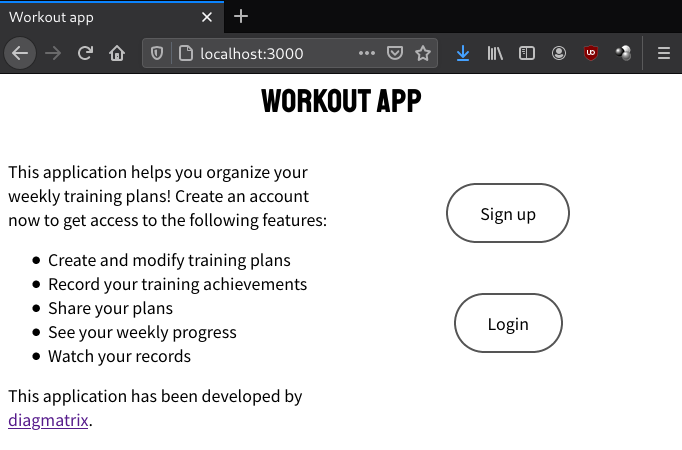
\includegraphics[scale=0.22]{landingpage.png}\end{center} \\
		\hline
		\multicolumn{5}{|c|}{\textbf{Registration} (\texttt{/register})} \\ 
		\hline 
		1.1 & Click "Sign up". & Registration page is loaded. & OK & 
		\begin{center}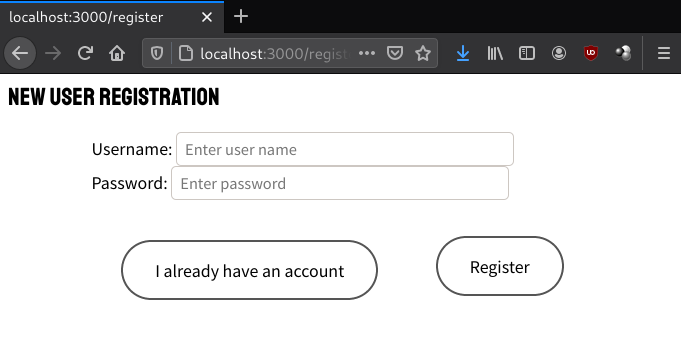
\includegraphics[scale=0.28]{register1.png}\end{center} \\
		\hline
		1.2 & Insert registration values. & User is registered and login page is loaded. & OK &
		\begin{center}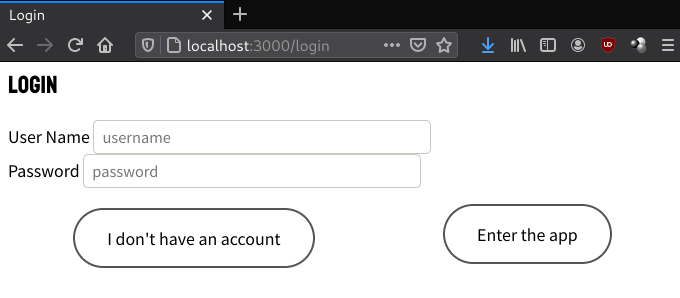
\includegraphics[scale=0.28]{register2-login1.png}\end{center} \\
		\hline
		1.3 & Insert registration values (username taken). & Registration page is reloaded with error message & OK &
		\begin{center}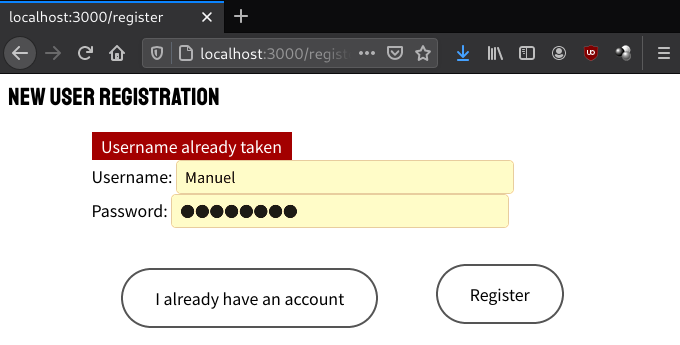
\includegraphics[scale=0.28]{register3.png}\end{center} \\
		\hline
	\end{tabular}
\end{table}
\newpage
\begin{table}[!h]
	\centering
	\begin{tabular}{|m{0.6cm}|m{2.9cm}|m{3.6cm}|m{1.1cm}|m{5.9cm}|}
		\hline
		\textbf{ID} & \textbf{Action} & \textbf{Expected output} & \textbf{Status} & \textbf{Evidence} \\
		\hline
		1.4 & Insert registration values (eLv\#9\$). & Registration page is reloaded with error message. & OK &
		\begin{center}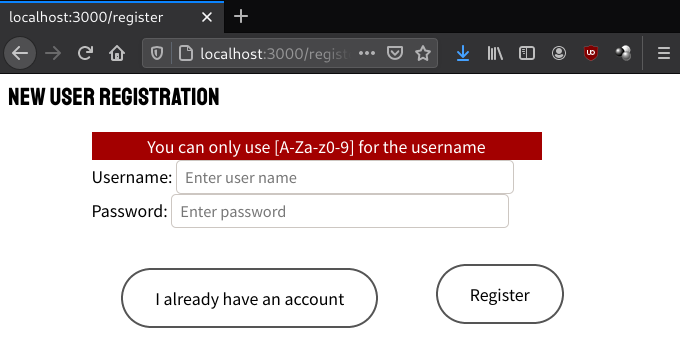
\includegraphics[scale=0.3]{register4.png}\end{center} \\
		\hline
		1.5 & Click "I already have an account". & Login page is loaded. & OK &
		\begin{center}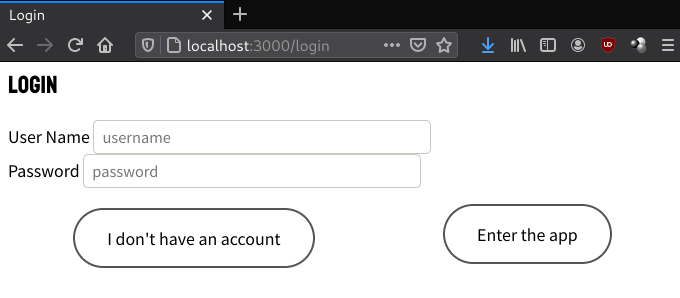
\includegraphics[scale=0.3]{register2-login1.png}\end{center} \\
		\hline
		\multicolumn{5}{|c|}{\textbf{Login} (\texttt{/login})} \\ 
		\hline
		2.1 & Insert correct login values. & Profile page is loaded. & OK &
		\begin{center}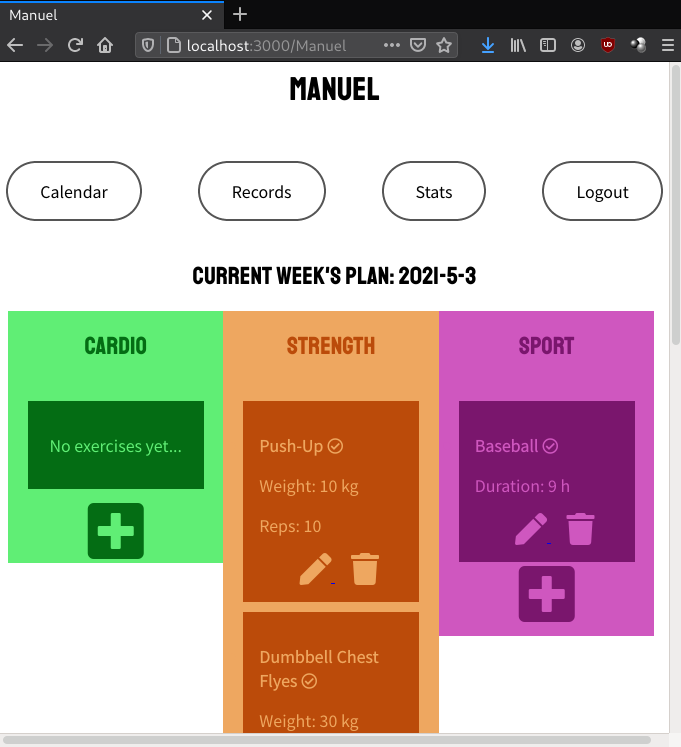
\includegraphics[scale=0.3]{login2-userpage1.png}\end{center} \\
		\hline
		2.2 & Insert incorrect login values (incorrect password). & Login page is reloaded. & OK &
		\begin{center}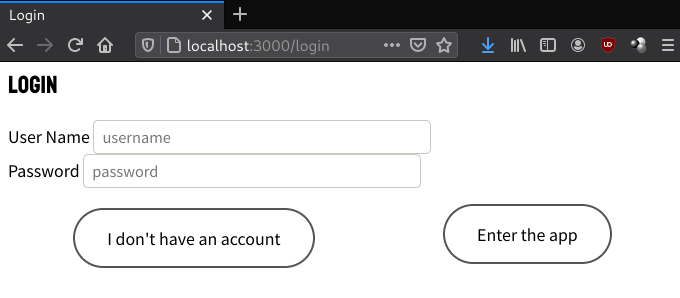
\includegraphics[scale=0.3]{register2-login1.png}\end{center} \\
		\hline
		2.3 & Insert incorrect login values (incorrect username). & Login page is reloaded. & OK &
		\begin{center}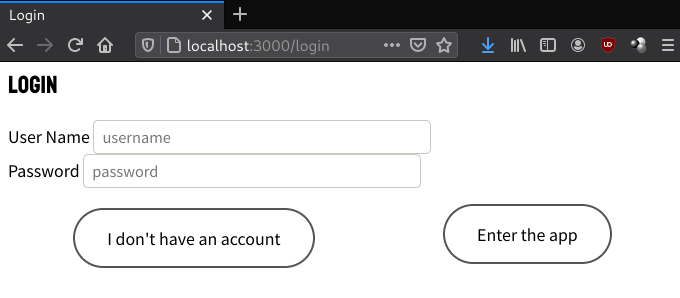
\includegraphics[scale=0.3]{register2-login1.png}\end{center} \\
		\hline
	\end{tabular}
\end{table}
\newpage
\begin{table}[!ht]
	\centering
	\begin{tabular}{|m{0.6cm}|m{2.9cm}|m{3.6cm}|m{1.1cm}|m{5.9cm}|}
		\hline
		\textbf{ID} & \textbf{Action} & \textbf{Expected output} & \textbf{Status} & \textbf{Evidence} \\
		\hline
		\multicolumn{5}{|c|}{\textbf{Profile page} (\texttt{/Manuel})} \\ 
		\hline
		3.1 & Access userpage URL. & Profile page is loaded. & OK &
		\begin{center}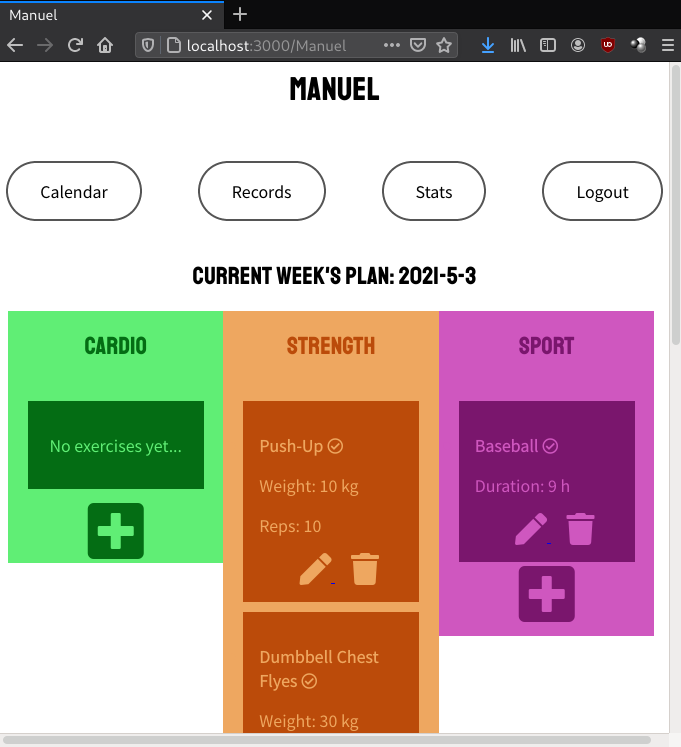
\includegraphics[scale=0.24]{login2-userpage1.png}\end{center} \\
		\hline
		3.2 & Access URL without logging in. & Login page is loaded instead. & OK &
		\begin{center}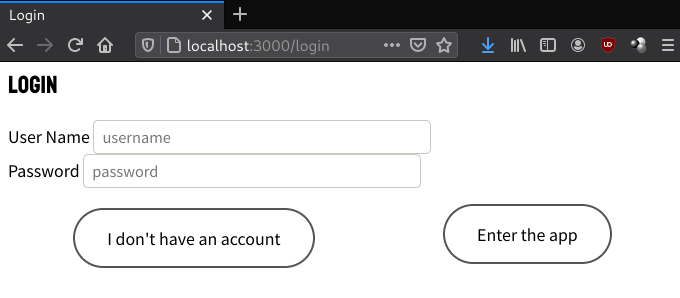
\includegraphics[scale=0.24]{register2-login1.png}\end{center} \\
		\hline
		3.3 & Access URL of a user while logged with another user. & Login page is loaded instead. & OK &
		\begin{center}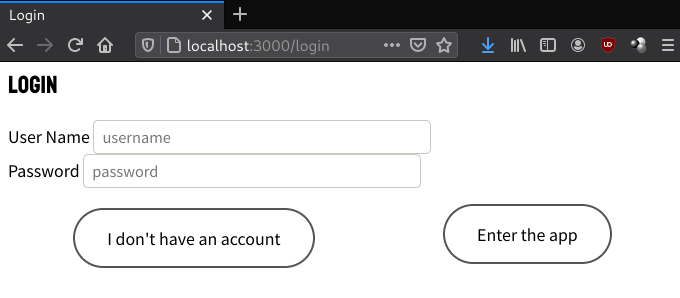
\includegraphics[scale=0.24]{register2-login1.png}\end{center} \\
		\hline
		3.4 & Click "Logout". & User is logged out and landing page is loaded. & OK &
		\begin{center}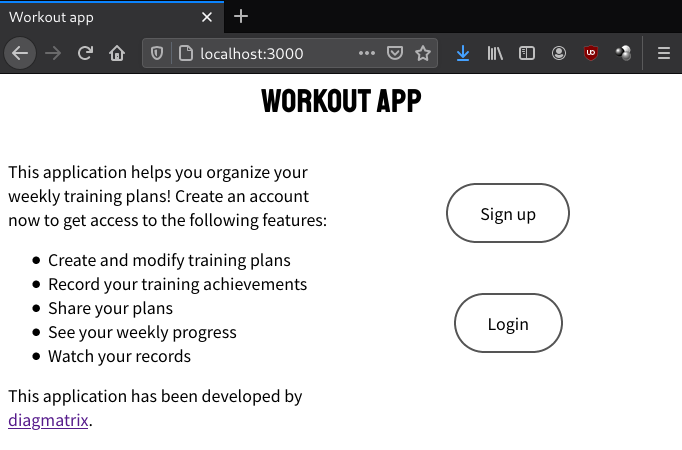
\includegraphics[scale=0.24]{landingpage.png}\end{center} \\
		\hline
		3.5 & Click "Calendar". & Calendar page is loaded. & OK &
		\begin{center}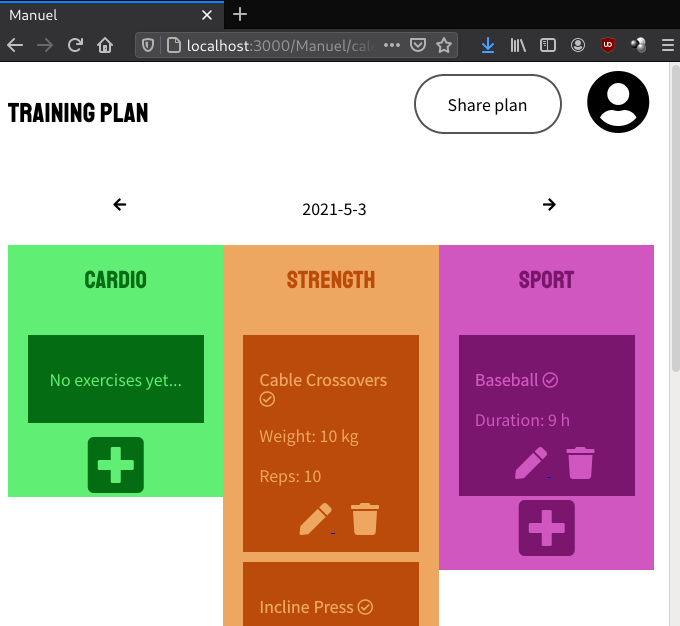
\includegraphics[scale=0.24]{userpage2-calendar1.png}\end{center} \\
		\hline
	\end{tabular}
\end{table}
\newpage
\begin{table}[!h]
	\centering
	\begin{tabular}{|m{0.6cm}|m{2.9cm}|m{3.6cm}|m{1.1cm}|m{5.9cm}|}
		\hline
		\textbf{ID} & \textbf{Action} & \textbf{Expected output} & \textbf{Status} & \textbf{Evidence} \\ 
		\hline
		3.6 & Click "Records". & Records page is loaded. & OK &
		\begin{center}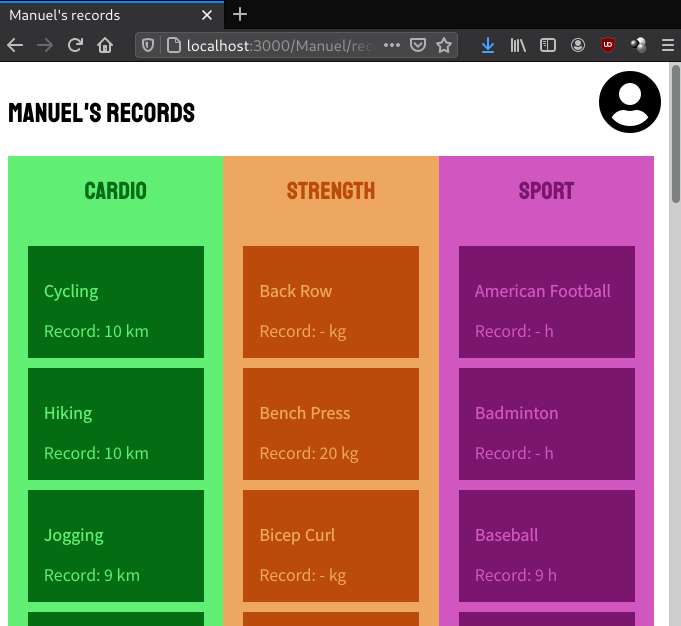
\includegraphics[scale=0.24]{records.png}\end{center} \\
		\hline
		3.7 & Click "Stats". & Stats page is loaded. & OK &
		\begin{center}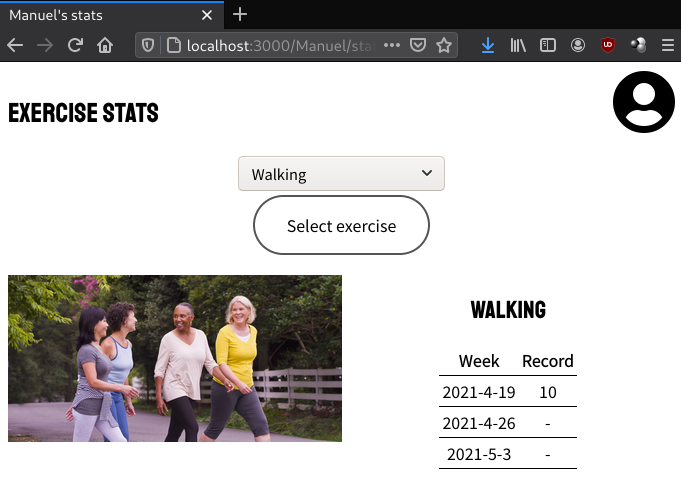
\includegraphics[scale=0.24]{userpage3-stats1.png}\end{center} \\
		\hline
		3.8 & Press the green "+" button in the cardio exercises column. & New cardio exercise page is loaded. & OK &
		\begin{center}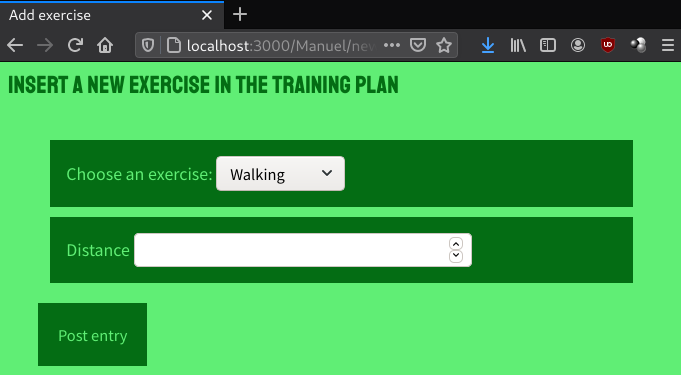
\includegraphics[scale=0.24]{userpage4-newcardio.png}\end{center} \\
		\hline
		3.9 & Complete the new exercise form and press "Post Entry". & Profile page is loaded with new exercise added to
		the current week's plan. & OK &
		\begin{center}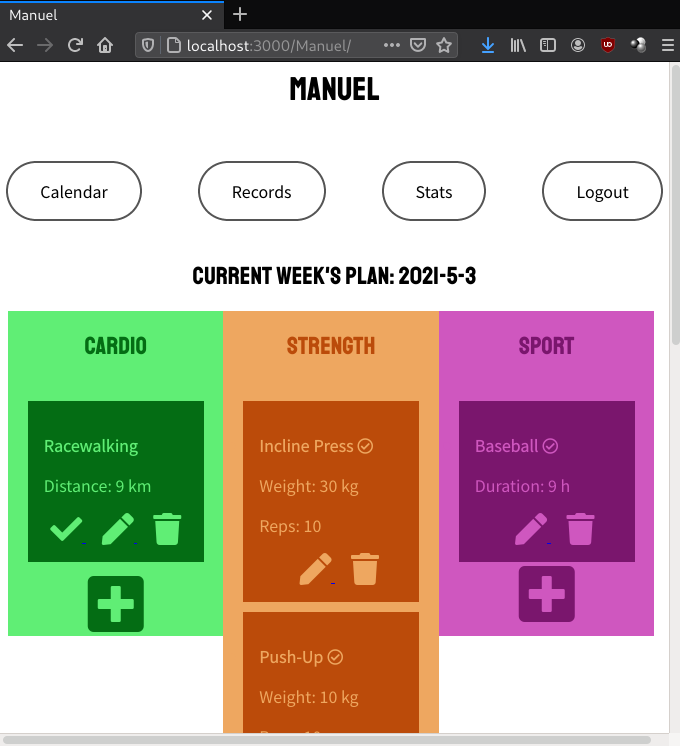
\includegraphics[scale=0.24]{newcardio-userpage6.png}\end{center} \\
		\hline
		3.10 & Press the purple pencil button under "Baseball". & Modify exercise page is loaded. & OK &
		\begin{center}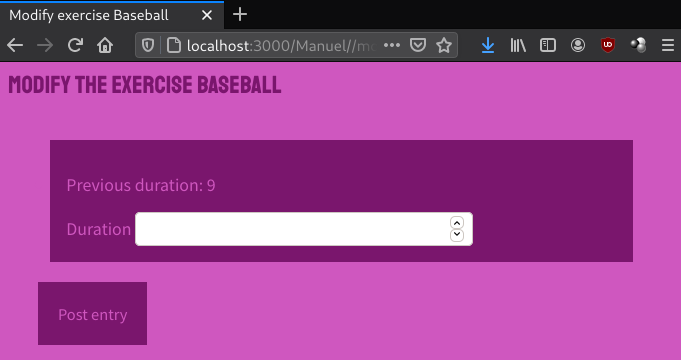
\includegraphics[scale=0.24]{userpage5-modifysport.png}\end{center} \\
		\hline
	\end{tabular}
\end{table}
\newpage
\begin{table}[!h]
	\centering
	\begin{tabular}{|m{0.6cm}|m{2.9cm}|m{3.6cm}|m{1.1cm}|m{5.9cm}|}
		\hline
		\textbf{ID} & \textbf{Action} & \textbf{Expected output} & \textbf{Status} & \textbf{Evidence} \\ 
		\hline
		3.11 & Complete the modification of the baseball exercise. & Profile page is loaded with the modification
		done and the exercise not marked as complete. & OK &
		\begin{center}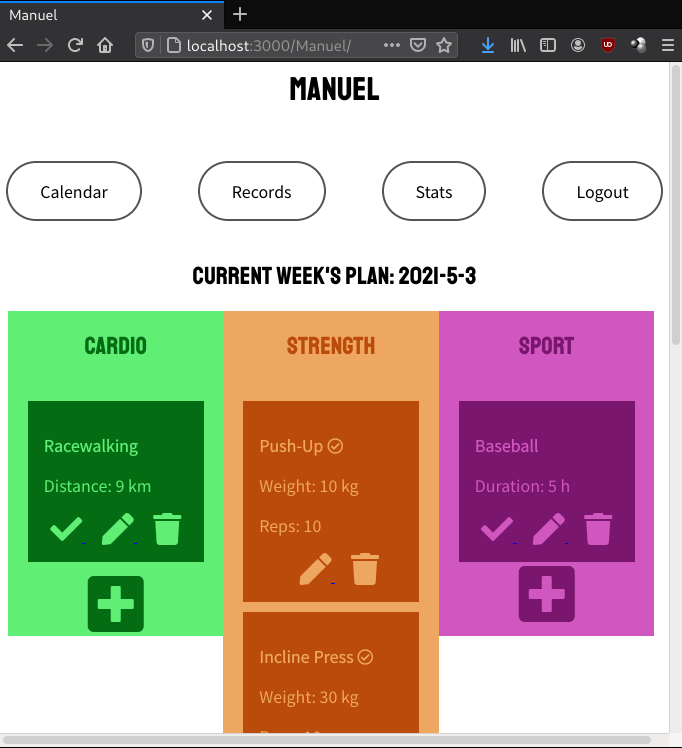
\includegraphics[scale=0.22]{modifysport-userpage7.png}\end{center} \\
		\hline
		3.12 & Press the orange trash button under "Push-Up". & Push-Up exercise is deleted from the plan. & OK &
		\begin{center}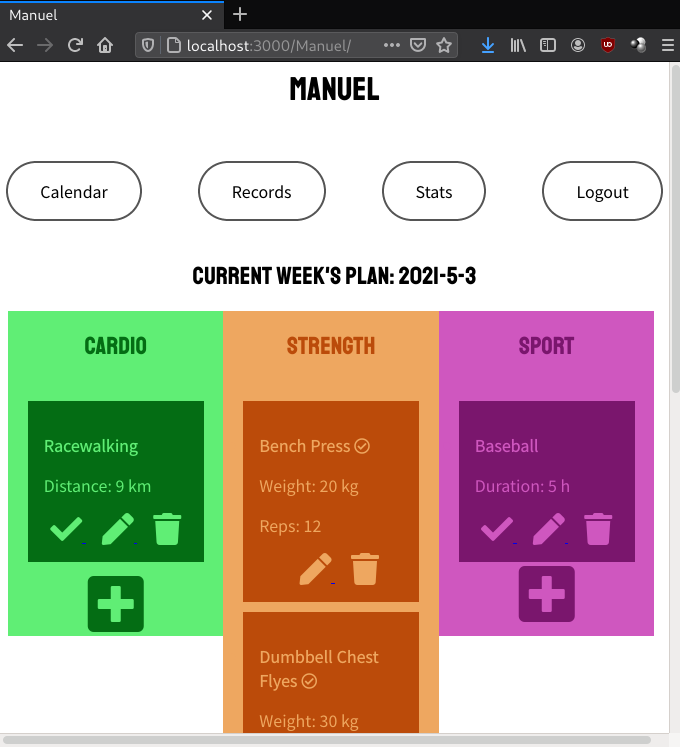
\includegraphics[scale=0.22]{userpage8.png}\end{center} \\
		\hline
		3.13 & Press the green check mark under "Racewalking". & "Racewalking" is marked as completed & OK &
		\begin{center}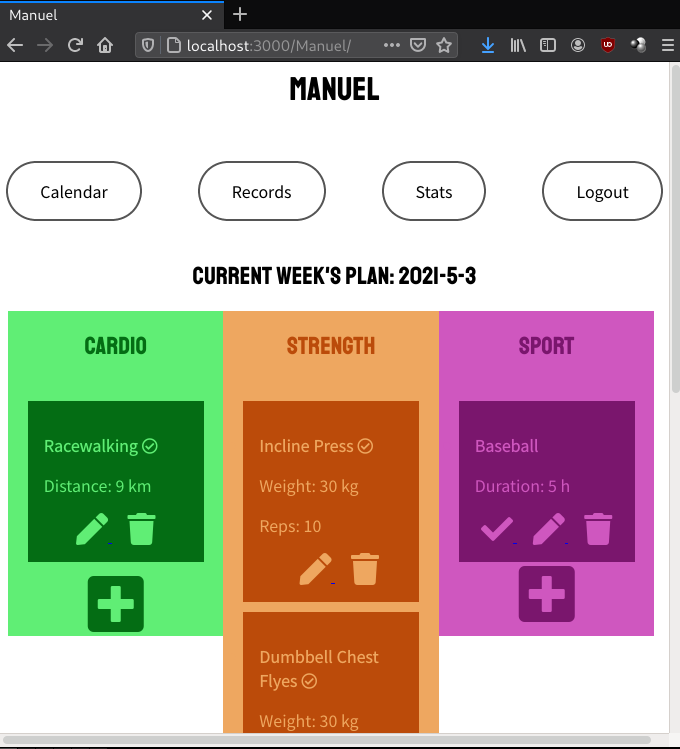
\includegraphics[scale=0.22]{userpage9.png}\end{center} \\
		\hline
		\multicolumn{5}{|c|}{\textbf{Records page} (\texttt{/Manuel/records})} \\ 
		\hline
		4.1 & Access records page URL. & Records page is loaded. & OK &
		\begin{center}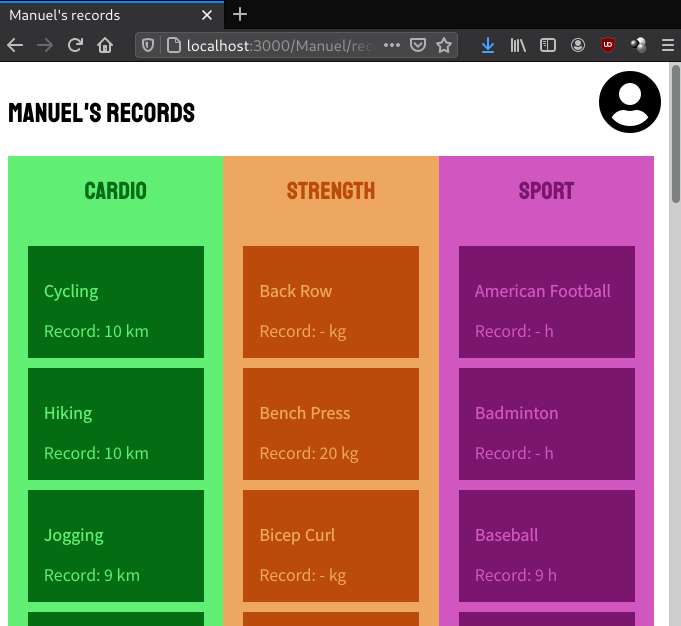
\includegraphics[scale=0.22]{records.png}\end{center} \\
		\hline
	\end{tabular}
\end{table}
\newpage
\begin{table}[!h]
	\centering
	\begin{tabular}{|m{0.6cm}|m{2.9cm}|m{3.6cm}|m{1.1cm}|m{5.9cm}|}
		\hline
		\textbf{ID} & \textbf{Action} & \textbf{Expected output} & \textbf{Status} & \textbf{Evidence} \\ 
		\hline
		4.2 & Access URL without logging in. & Login page is loaded instead. & OK &
		\begin{center}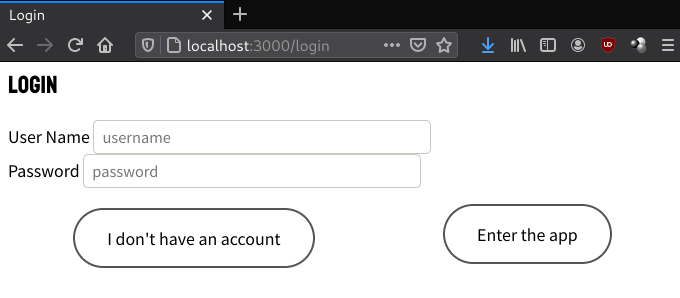
\includegraphics[scale=0.22]{register2-login1.png}\end{center} \\
		\hline
		4.3 & Access URL of a user while logged with another user. & Login page is loaded instead. & OK &
		\begin{center}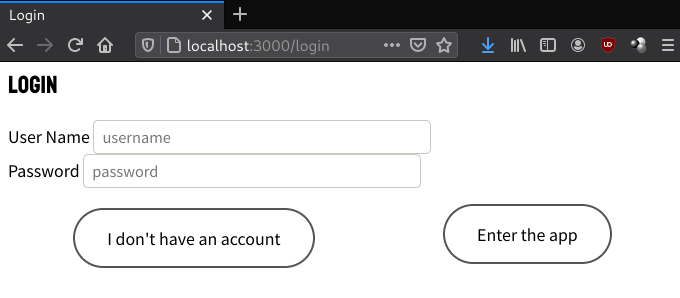
\includegraphics[scale=0.22]{register2-login1.png}\end{center} \\
		\hline
		4.4 & Click "avatar" image. & Profile page is loaded. & OK &
		\begin{center}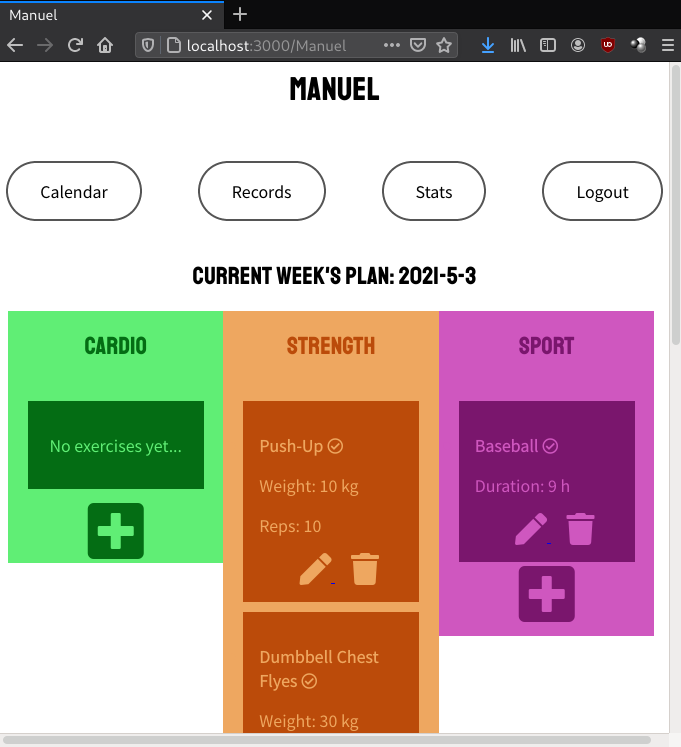
\includegraphics[scale=0.22]{login2-userpage1.png}\end{center} \\
		\hline
		\multicolumn{5}{|c|}{\textbf{Stats page} (\texttt{/Manuel/stats})} \\ 
		\hline
		5.1 & Access records page URL. & Stats page is loaded. & OK &
		\begin{center}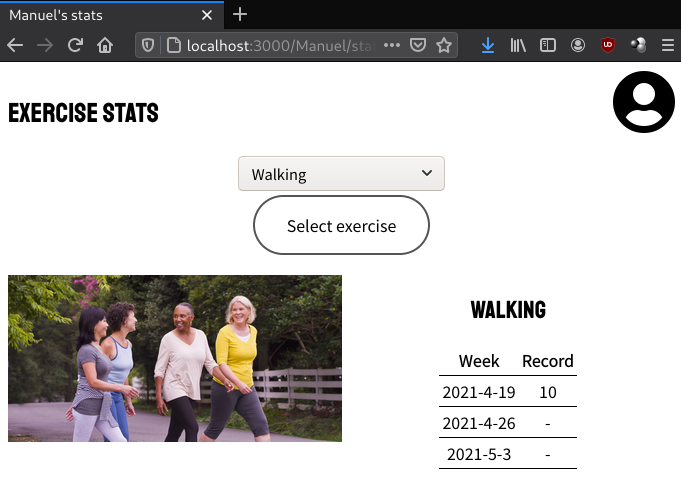
\includegraphics[scale=0.22]{userpage3-stats1.png}\end{center} \\
		\hline
		5.2 & Access URL without logging in. & Login page is loaded instead. & OK &
		\begin{center}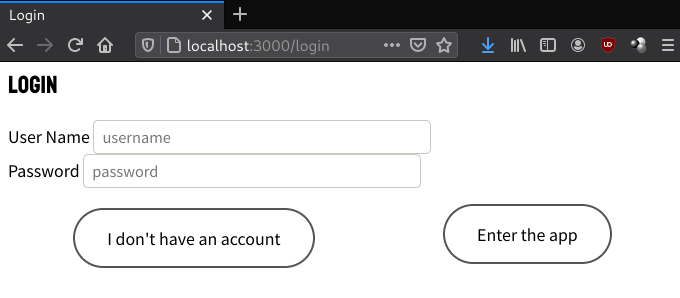
\includegraphics[scale=0.22]{register2-login1.png}\end{center} \\
		\hline
		5.3 & Access URL of a user while logged with another user. & Login page is loaded instead. & OK &
		\begin{center}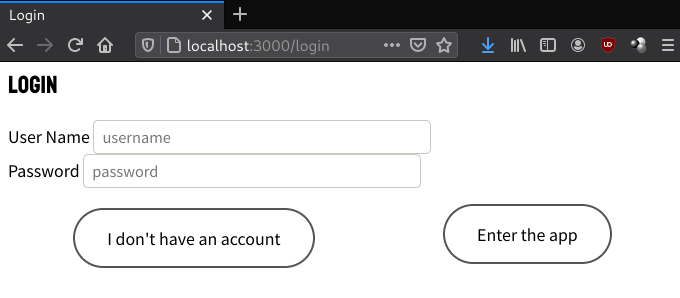
\includegraphics[scale=0.22]{register2-login1.png}\end{center} \\
		\hline
	\end{tabular}
\end{table}
\newpage
\begin{table}[!h]
	\centering
	\begin{tabular}{|m{0.6cm}|m{2.9cm}|m{3.6cm}|m{1.1cm}|m{5.9cm}|}
		\hline
		\textbf{ID} & \textbf{Action} & \textbf{Expected output} & \textbf{Status} & \textbf{Evidence} \\ 
		\hline
		5.4 & Select another exercise (Push-Up). & Stats page is loaded with Push-Up exercise. & OK &
		\begin{center}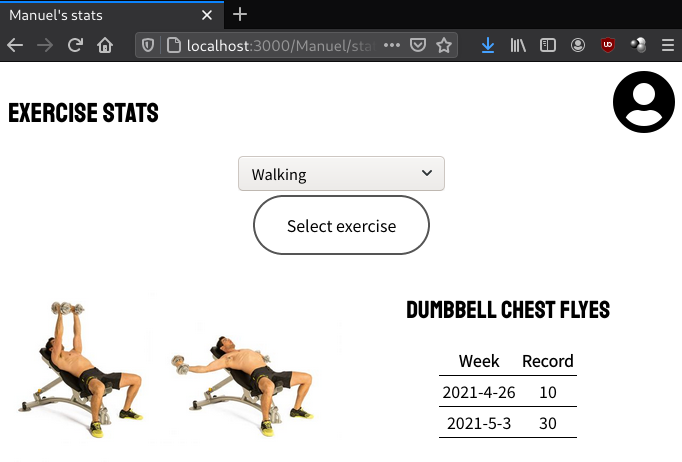
\includegraphics[scale=0.22]{stats2.png}\end{center} \\
		\hline
		\multicolumn{5}{|c|}{\textbf{Calendar page} (\texttt{/Manuel/calendar})} \\ 
		\hline
		6.1 & Access calendar page URL. & Calendar page is loaded with current week & OK &
		\begin{center}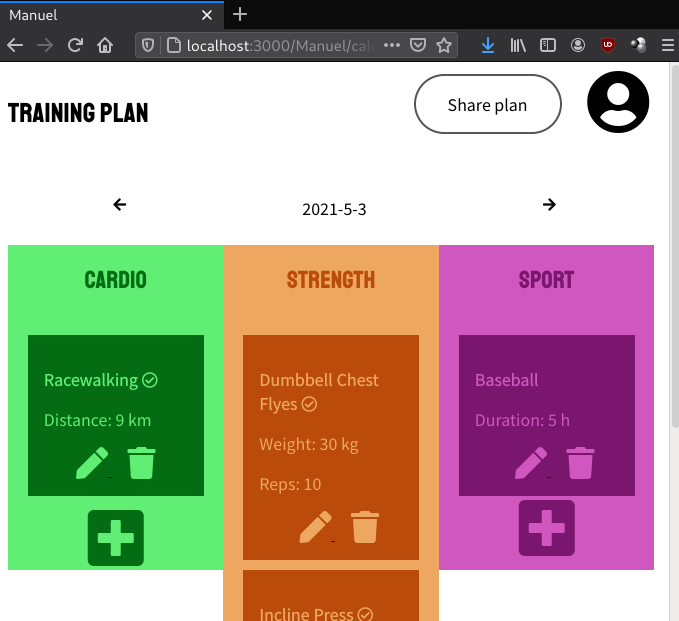
\includegraphics[scale=0.22]{calendar1.png}\end{center} \\
		\hline
		6.2 & Access URL without logging in. & Login page is loaded instead. & OK &
		\begin{center}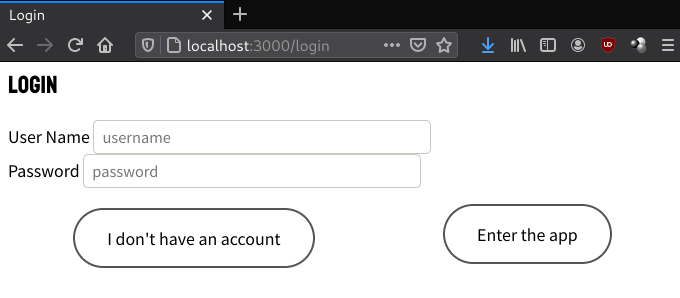
\includegraphics[scale=0.22]{register2-login1.png}\end{center} \\
		\hline
		6.3 & Access URL of a user while logged with another user. & Login page is loaded instead. & OK &
		\begin{center}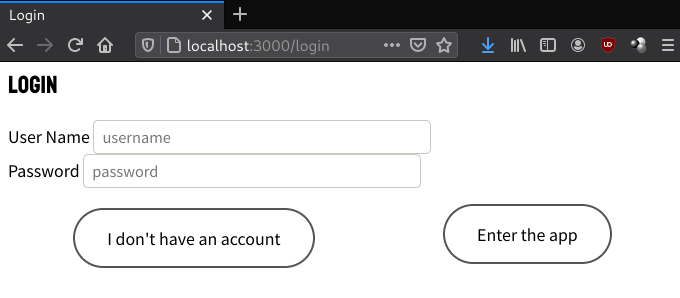
\includegraphics[scale=0.22]{register2-login1.png}\end{center} \\
		\hline
		6.4 & Click "avatar" image. & Profile page is loaded. & OK &
		\begin{center}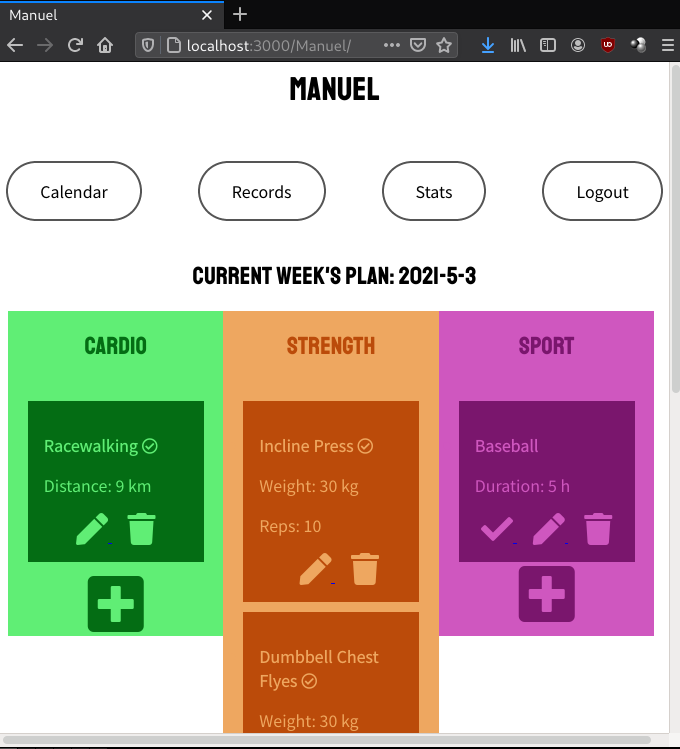
\includegraphics[scale=0.22]{userpage9.png}\end{center} \\
		\hline
	\end{tabular}
\end{table}
\newpage
\begin{table}[!h]
	\centering
	\begin{tabular}{|m{0.6cm}|m{2.9cm}|m{3.6cm}|m{1.1cm}|m{5.9cm}|}
		\hline
		\textbf{ID} & \textbf{Action} & \textbf{Expected output} & \textbf{Status} & \textbf{Evidence} \\ 
		\hline
		6.5 & Change week to an unplanned week (10/05). & Calendar page is loaded with no plan. & OK &
		\begin{center}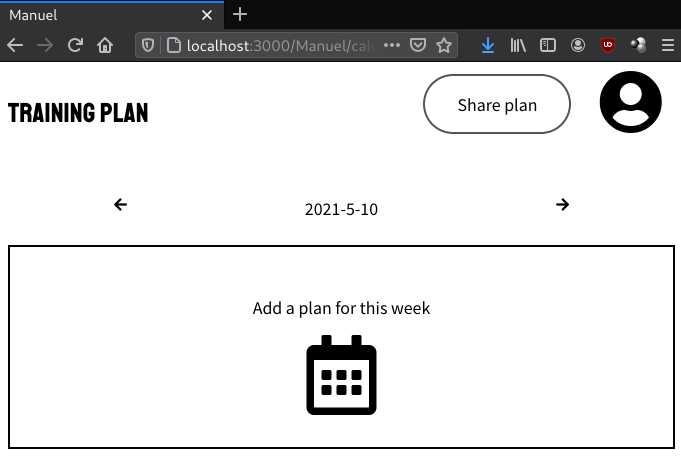
\includegraphics[scale=0.22]{calendar2.png}\end{center} \\
		\hline
		6.6 & Change week to a planned week (19/04). & Calendar page is loaded with that week's plan. & OK &
		\begin{center}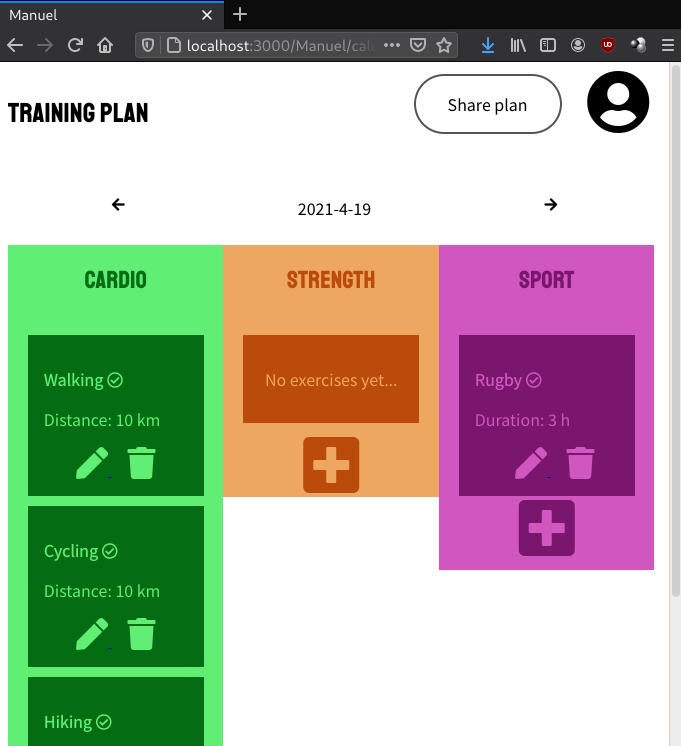
\includegraphics[scale=0.22]{calendar3.png}\end{center} \\
		\hline
		6.7 & Click "Share plan" (03/05). & Sharing plan page loads with link to the shared plan page. & OK &
		\begin{center}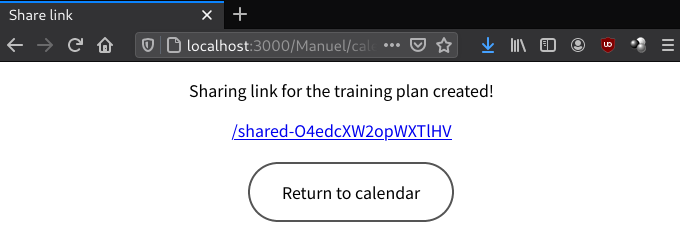
\includegraphics[scale=0.22]{calendar4-shareplan.png}\end{center} \\
		\hline
		6.8 & Click "Return to calendar". & Calendar page is loaded. & OK &
		\begin{center}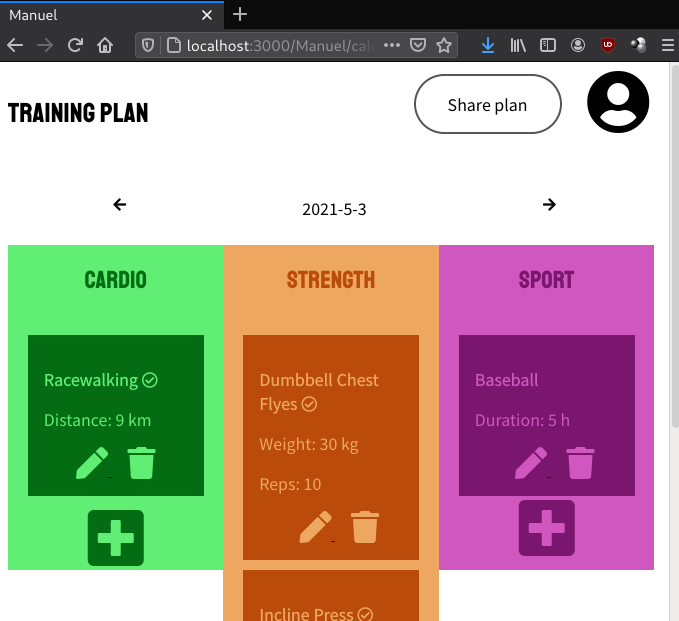
\includegraphics[scale=0.22]{calendar1.png}\end{center} \\
		\hline
		6.9 & Press the purple trash button under "Baseball". & Baseball exercise is removed from the plan. & OK &
		\begin{center}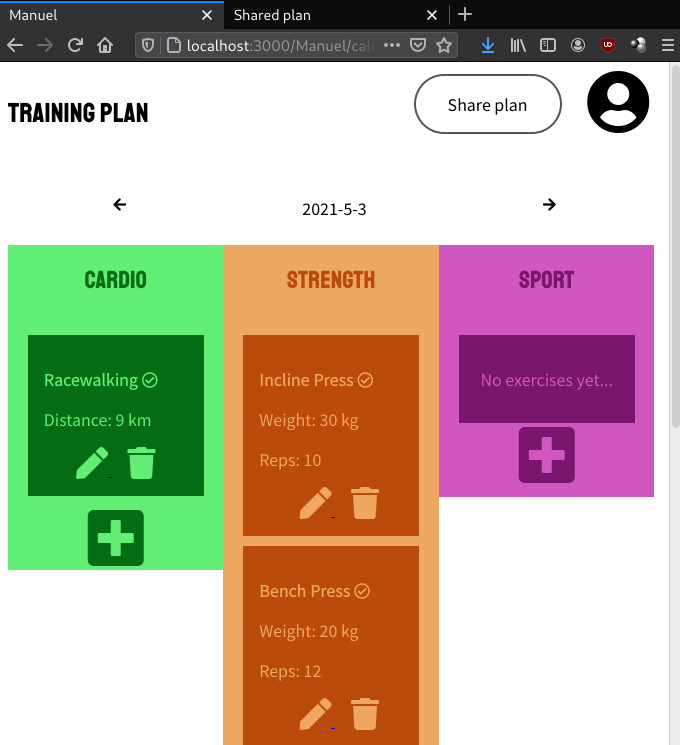
\includegraphics[scale=0.22]{calendar4.png}\end{center} \\
		\hline
	\end{tabular}
\end{table}
\newpage
\begin{table}[!h]
	\centering
	\begin{tabular}{|m{0.6cm}|m{2.9cm}|m{3.6cm}|m{1.1cm}|m{5.9cm}|}
		\hline
		\textbf{ID} & \textbf{Action} & \textbf{Expected output} & \textbf{Status} & \textbf{Evidence} \\ 
		\hline
		6.10 & Press the purple "+" button in the sport exercises column. & New sport exercise page is loaded. & OK &
		\begin{center}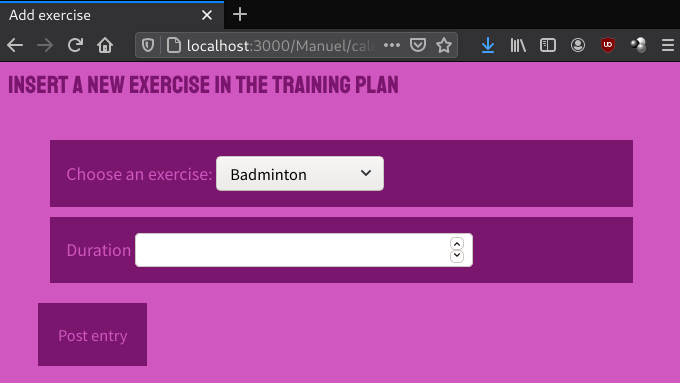
\includegraphics[scale=0.22]{newsport.png}\end{center} \\
		\hline
		6.11 & Complete the new exercise form and press "Post entry". & Calendar page is loaded with the new exercise
		added to the plan. & OK &
		\begin{center}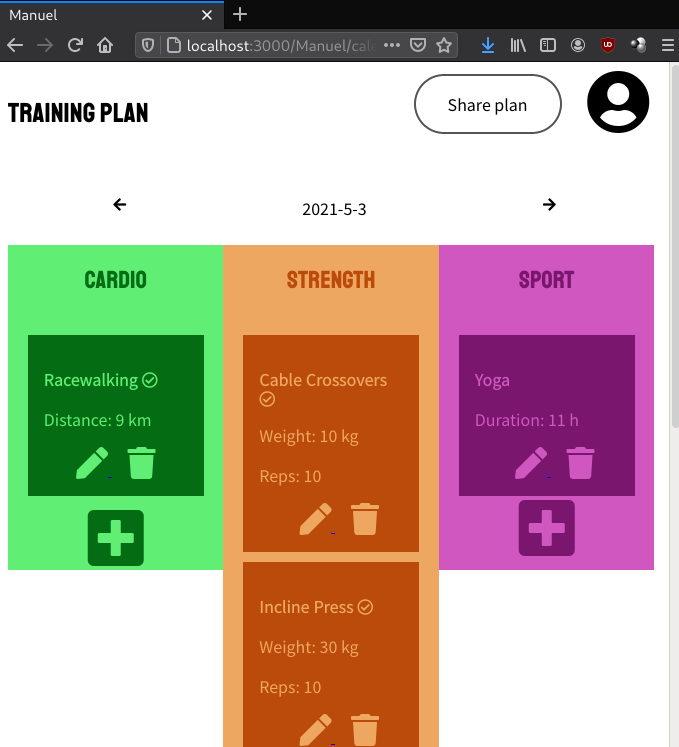
\includegraphics[scale=0.22]{calendar5.png}\end{center} \\
		\hline
		6.12 & Press the orange pencil under "Cable Crossovers". & Exercise modification page is loaded. & OK &
		\begin{center}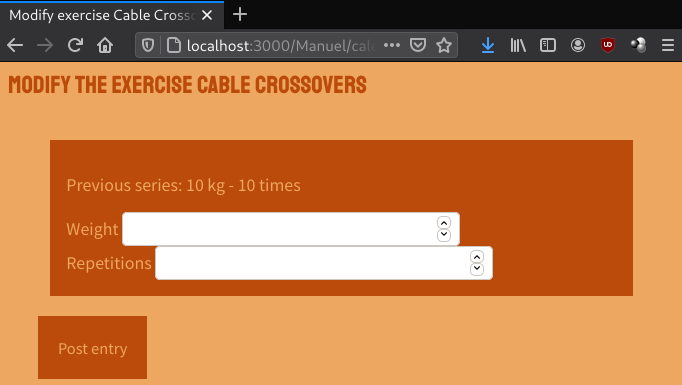
\includegraphics[scale=0.22]{modifystr.png}\end{center} \\
		\hline
		6.13 & Complete the modification form and press "Post entry". & Calendar page is loaded with the modified exercise, 
		marked as uncompleted. & OK &
		\begin{center}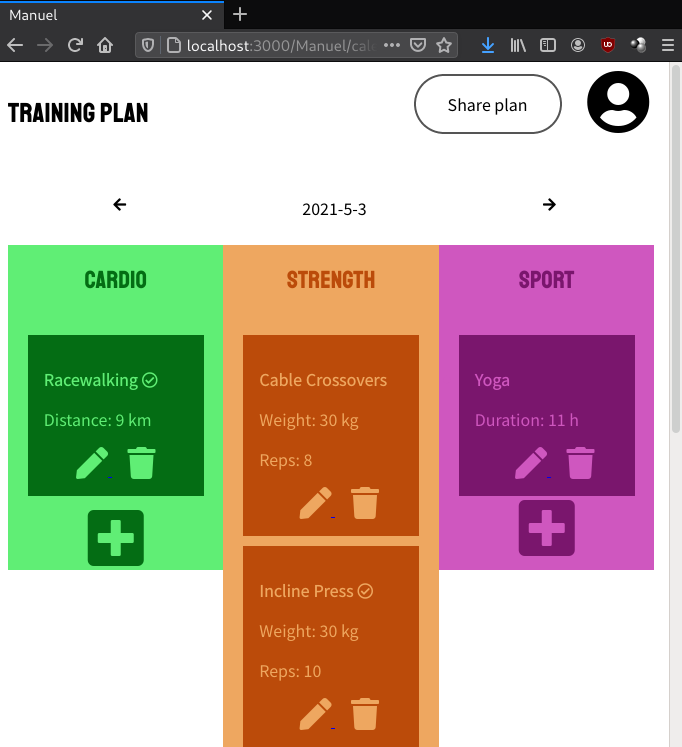
\includegraphics[scale=0.22]{calendar6.png}\end{center} \\
		\hline
		6.14 & Calendar icon under "Add plan for this week" is pressed (10/05). & Create new plan page is loaded. & OK &
		\begin{center}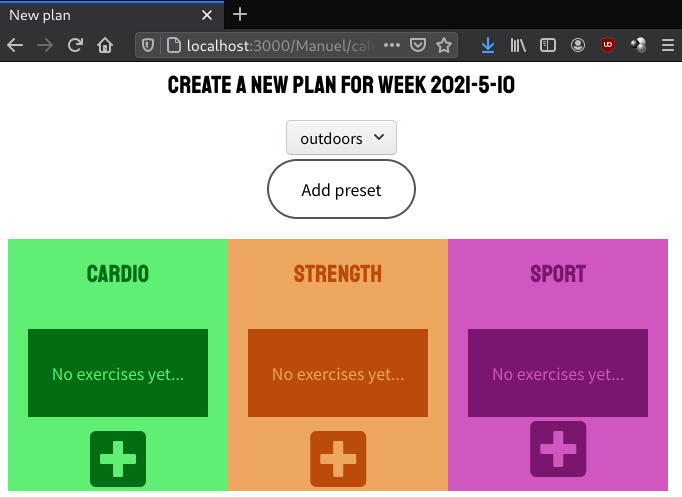
\includegraphics[scale=0.22]{newplan1.png}\end{center} \\
		\hline
	\end{tabular}
\end{table}
\newpage
\begin{table}[!h]
	\centering
	\begin{tabular}{|m{0.6cm}|m{2.9cm}|m{3.6cm}|m{1.1cm}|m{5.9cm}|}
		\hline
		\textbf{ID} & \textbf{Action} & \textbf{Expected output} & \textbf{Status} & \textbf{Evidence} \\ 
		\hline
		\multicolumn{5}{|c|}{\textbf{New plan page} (\texttt{/Manuel/calendar/2021-5-10-new})} \\ 
		\hline
		7.1 & Access new plan URL. & New plan page is loaded. & OK &
		\begin{center}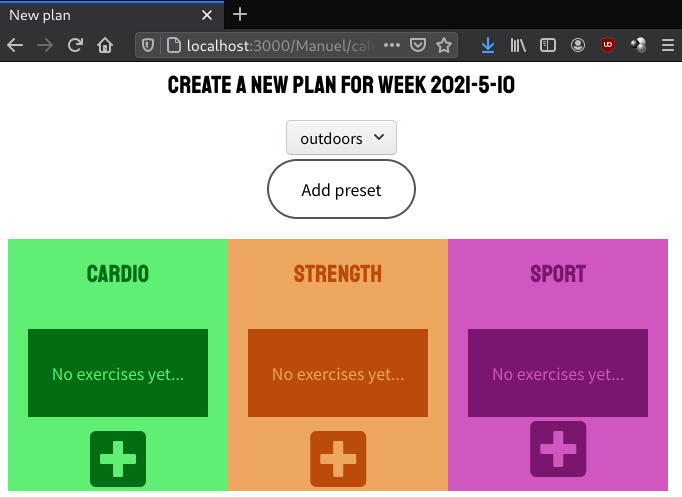
\includegraphics[scale=0.22]{newplan1.png}\end{center} \\
		\hline
		7.2 & Access URL without logging in. & Login page is loaded instead. & OK &
		\begin{center}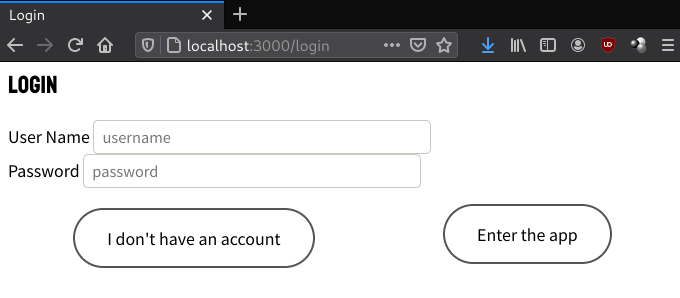
\includegraphics[scale=0.22]{register2-login1.png}\end{center} \\
		\hline
		7.3 & Access URL of a user while logged with another user. & Login page is loaded instead. & OK &
		\begin{center}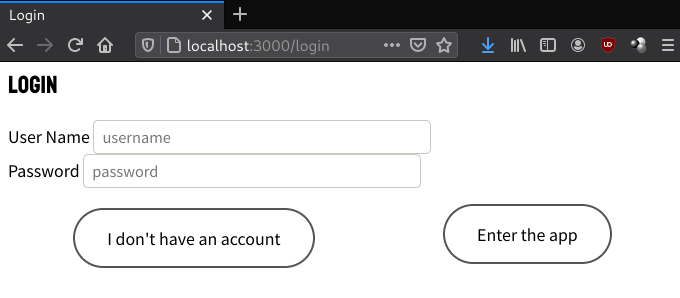
\includegraphics[scale=0.22]{register2-login1.png}\end{center} \\
		\hline
		7.4 & Add exercises (less than minimum of three). & Plan is reloaded with exercises added. & OK & 
		\begin{center}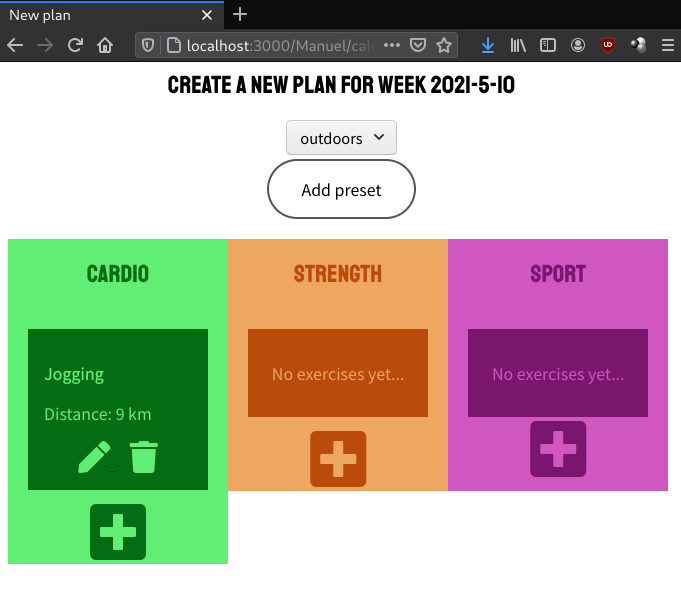
\includegraphics[scale=0.22]{newplan3.png}\end{center} \\
		\hline
		7.5 & Delete exercises. & Exercises are deleted. & OK & \textit{(Same page but without those exercises)} \\
		\hline
		7.6 & Modify exercises. & Exercises are modified. & OK & \textit{(Same page but with those exercises modified)} \\
		\hline
		7.7 & Select "outdoors" preset. & Preset exercises added to the plan. & OK &
		\begin{center}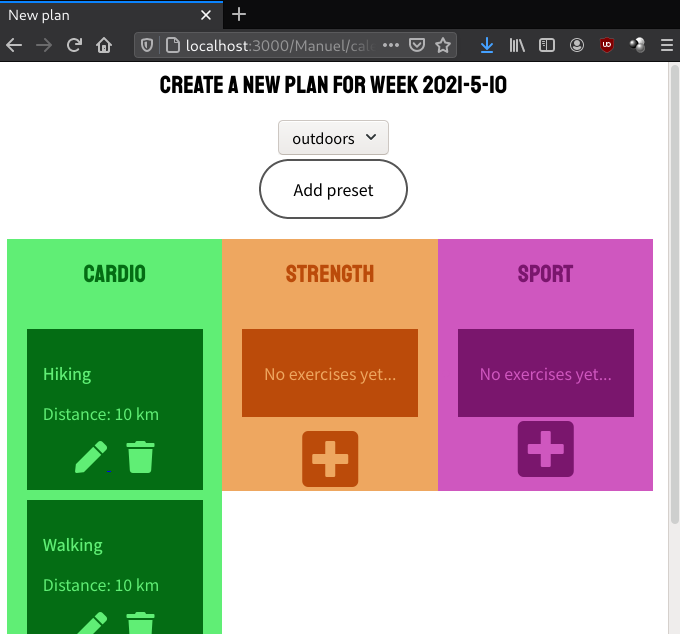
\includegraphics[scale=0.22]{newplan2.png}\end{center} \\
		\hline
	\end{tabular}
\end{table}
\newpage
\begin{table}[!h]
	\centering
	\begin{tabular}{|m{0.6cm}|m{2.9cm}|m{3.6cm}|m{1.1cm}|m{5.9cm}|}
		\hline
		\textbf{ID} & \textbf{Action} & \textbf{Expected output} & \textbf{Status} & \textbf{Evidence} \\ 
		\hline
		7.8 & Add exercises (more than two). & Exercises are added and "Generate plan" button appears. & OK &
		\begin{center}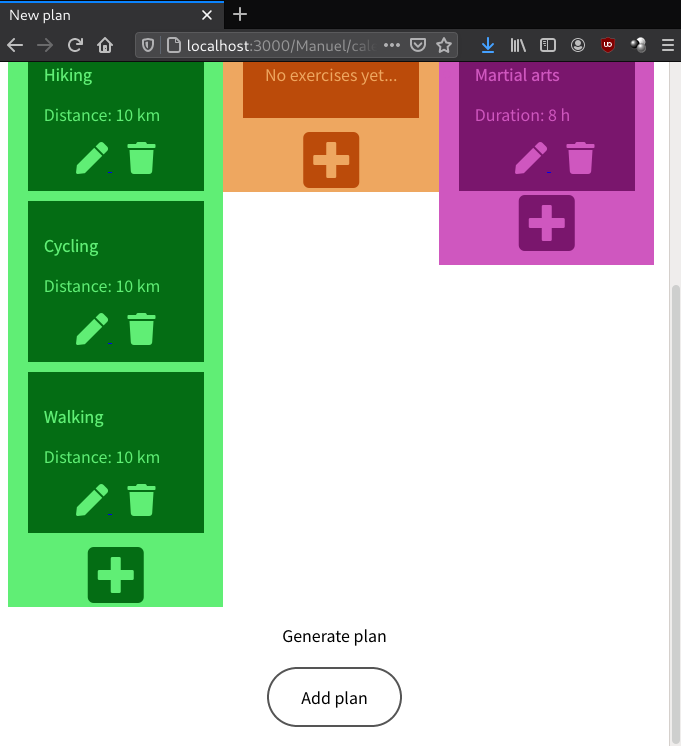
\includegraphics[scale=0.18]{newplan4.png}\end{center} \\
		\hline
		7.9 & Press "Generate plan". & Calendar page is loaded with that weekly plan. & OK &
		\begin{center}\includegraphics[scale=0.18]{newplan5.png}\end{center} \\
		\hline
		\multicolumn{5}{|c|}{\textbf{Shared plan page}} \\ 
		\hline
		8.1 & Access shared plan URL logged in (from test 6.7). & Shared plan page is loaded. & OK & 
		\begin{center}\includegraphics[scale=0.18]{shared1.png}\end{center} \\
		\hline
		8.2 & Access shared plan URL not logged in (from test 6.7). & Shared plan page is loaded. & OK & 
		\begin{center}\includegraphics[scale=0.18]{shared1.png}\end{center} \\
		\hline
		8.3 & Access invalid shared plan URL (\texttt{/shared-} \texttt{thisisnot}). & Error page is loaded. & OK & 
		\begin{center}\includegraphics[scale=0.22]{shared2.png}\end{center} \\
		\hline
	\end{tabular}
\end{table}
\newpage

\subsubsection*{Summary of tests}
All tests made to each page passed as expected. The functionalities regarding training plan manipulation (adding exercises,
modifying exercises, completing exercises and deleting exercises) were tested anywhere they could: in the profile page with
the current week's weekly plan; in the calendar page, as existing weekly plans can be modified; and in the training plan
creation page.
\newline\newline
Possibilities that were not tested:
\begin{itemize}
	\item Trying to access training plan manipulation pages (for example, \texttt{/Manuel/new-cardio}) while not logged in.
	Trying to do this should redirect the user to the login page.
	\item Trying to access training plan manipulation pages while logged with another user (for example, while logged as
	"Manuel", trying to access \texttt{/Elvira/new-sport}). This should be permitted, but when the user tries to post the
	exercise, the login page should load instead.
\end{itemize}
Possibilities that cannot be tested:
\begin{itemize}
	\item Completing exercises for weeks that are not the current one. The application does not allow that to happen, as the
	check mark button is only present in the profile page's plan.
	\item Deleting exercises from an existing plan that has only exercises in it. The application hides the deletion button
	if the number of exercises is less than four.
\end{itemize}

\newpage
\section{Application security}

\subsection{Cookies}
The application uses one cookie, to store the session of a user. This is used so the user does not have to log in every time
they try to access features restricted to registered users. The sessions are implemented using the package named 
\textbf{express-session}.
\newline\newline
When the application is loaded the first time(\texttt{localhost:3000/}), a cookie is created. This cookie is named 
\textbf{connect.sid}, and does not change its value when logging in and out with different users. When you delete the session 
cookie using the developer tools of the web browser (Mozilla Firefox in my specific case), the application treats this as if 
the user was logged out, the login page is rendered, and a new session cookie is created. This means that users' information 
(their weekly plans) cannot be accessed if the cookie is destroyed.
\newline\newline
When you close the page, however, the cookie is not destroyed. This means that if a user closes the page and does not log out,
any other person that accessed the page with that cookie during the lifetime of it. As stated in the \textbf{express-session}
documentation\footnote{\url{https://www.npmjs.com/package/express-session\#cookieexpires}}, if no expiring date or maximum age
is set, the client takes the responsibility. In this application, a maximum age of 30 minutes is set for the cookie.
\newline\newline
By default, session cookies created by the package are httpOnly, and they can be made secure if it is specified when created.
A cookie used by the application has the following values:
\begin{lstlisting}
connect.sid:"s%3AYnwE7-vlb0Mx7j58hphWvbx9lpcqTJhp.rHVmVaIssceCh19EteAIdYsVT%2ByeFbyx2p%2BaRw7T1rc"
Created:"Sat, 08 May 2021 11:53:03 GMT"
Domain:"localhost"
Expires/Max-Age:"Sat, 08 May 2021 12:34:57 GMT"
HostOnly:true
HttpOnly:true
Last Accessed:"Sat, 08 May 2021 11:53:03 GMT"
Path:"/"
SameSite:"None"
Secure:false
Size:95
\end{lstlisting}
The secure flag could also be used, but the package documentation warns about using secure flags and HTTP connections
\footnote{\url{https://www.npmjs.com/package/express-session\#cookiesecure}}. Because I am using an HTTP connection to run the
application, then the cookie would not be sent back to the server if I used the flag, rendering the application useless, as no
user could leave the login page.

\subsection{User input and passwords}
The application only allows user input in the following cases:
\begin{itemize}[noitemsep]
	\item At registration.
	\item At login.
	\item Adding and modifying exercises.
\end{itemize}
I implemented the following measures to limit the user input in the application:
\begin{enumerate}
	\item Only alphanumeric values are valid in the application. Furthermore, the usernames "calendarDB" and "manager" are also
	disabled, because they are variable names of the calendar and user databases.
	\item Exercise names are fixed values, and the forms only allow number inputs in the fields.
\end{enumerate}
With this measures, user input is very limited. This also may limit the option of possible exercises. This is easily solved, as
the addition of new exercises only consists on adding the names into their corresponding array in the module \textbf{auxiliaries},
the corresponding category form, and in the stats page form.
\newline\newline
The passwords are stored after passing a hashing algorithm with ten salt rounds, using \textbf{bcrypt}. When a password is typed,
it is hashed and then compared to the stored one. The usernames and passwords are stored in a specific file, separated from the
database files where most of the operations take place.

\subsection{Crashes and unknown links}

There are two instances in which the application may crash: The first one, if the request is not properly handled, is a very simple
message that states "Internal Server Error". This does not reveal any information. The second one is if the crash resides in the
server (for example, if we type for example \texttt{/Manuel/modify-cardio-5aopogDRemysIds5}) and the cardio exercise with ID
\textbf{5aopogDRemysIds5} does not exist. The browser in this case shows the "Unable to connect" error, whilst in the console the
specific reason for the crash is shown. This means that the only way for a user to have access to information is by having access
to the console logs.
\newline\newline
For unknown links, if the URL is just \texttt{/<text>}, then the application will interpret this as trying to access the profile
page of user "text", and redirect to the login page (for example, trying to access \texttt{/modify-sport-55} will make the
application think you want to access the profile page of user "modify-sport-55"). The rest of the unmanaged links are redirected
to a simple 404 error page.

\end{document}